\newcommand{\institut}{}
\newcommand{\fachgebiet}{Regelungstechnik}
\newcommand{\veranstaltung}{Praktikum Grundlagen der Regelungstechnik}
\newcommand{\pdfautor}{Dirk Barbendererde (321 836), Boris Henckell (325 779)}
\newcommand{\autor}{Dirk Barbendererde (321 836)\\ Boris Henckell (325 779)}
\newcommand{\pdftitle}{Praktikum\ Regelungstechnik\ Versuch\ 2a}
\newcommand{\prototitle}{Praktikum Regelungstechnik \\ Versuch 2a}
\newcommand{\aufgabe}{}

\newcommand{\gruppe}{Gruppe: G1 Di 12-14}
\newcommand{\betreuer}{Betreuer: Behrang Monajemi Nejad}



\input{../../packages/tu_header_9}
%\begin{document}

% \lstlistoflistings
\definecolor{darkgray}{rgb}{0.95,0.95,0.95}
\lstset{language=Scilab}
\lstset{inputencoding=utf8}
%\lstset{extendedchars=true} % Umlaute an der richtigen stelle und nicht am Anfang ausgeben
\lstset{backgroundcolor=\color{darkgray}}
\lstset{numbers=left, numberstyle=\tiny, stepnumber=1, numbersep=7pt, breaklines=true}
\lstset{keywordstyle=\color{red}\bfseries\emph}
\lstset{
breaklines,
numbers=left,
frame=single,
xleftmargin=-2cm,
xrightmargin=-1.5cm
}
% enables UTF-8 in source code: (dirty, dirty hack)
\lstset{literate=
    %Deutsch
    {ä}{{\"a}}1 {ö}{{\"o}}1 {ü}{{\"u}}1 {Ä}{{\"A}}1 {Ö}
    {{\"O}}1 {Ü}{{\"U}}1 {ß}{\ss}1
    %Türkisch
    {â}{{\^{a}}}1 {Â}{{\^{A}}}1 {ç}{{\c{c}}}1 {Ç}{{\c{C}}}1 {ğ}{{\u{g}}}1 {Ğ}{{\u{G}}}1 {ı}{{\i}}1 {İ}{{\.{I}}}1 {ö}{{\"o}}1 {Ö}{{\"O}}1 {ş}{{\c{s}}}1
    {Ş}{{\c{S}}}1 {ü}{{\"u}}1 {Ü}{{\"U}}1
    %Polish
    {ą}{{\k{a}}}1 {ć}{{\'c}}1 {ę}{{\k{e}}}1 {ł}{{\l{}}}1 {ń}{{\'n}}1 {ó}{{\'o}}1 {ś}{{\'s}}1 {ż}{{\.z}}1 {ź}{{\'z}}1 {Ą}{{\k{A}}}1 {Ć}{{\'C}}1
    {Ę}{{\k{E}}}1 {Ł}{{\L{}}}1 {Ń}{{\'N}}1 {Ó}{{\'O}}1 {Ś}{{\'S}}1 {Ż}{{\.Z}}1 {Ź}{{\'Z}}1
    %Spanish
    {á}{{\'a}}1 {é}{{\'e}}1 {í}{{\'i}}1 {ó}{{\'o}}1 {ú}{{\'u}}1 {ñ}{{\~n}}1
}

%     \lstinputlisting{./praktikum6.sce}



%---------------------------------------------------------------------
%---------------------------------------------------------------------
%---------------------------------------------------------------------

\section{Vorbereitungsaufgaben}
\begin{quote}
	\hspace{-2em}
	\subsection{Linearisierung}
    Aufgabe:\\
    Linearisieren Sie das nichtlineare Modell um die Ruhelage ($z, \varphi$) = ($0, 0$) und berechnen Sie die
    Transferfunktion von der Stellgröße $u$ zum Ausgang $\varphi$. Skizzieren Sie die Pol-/Nullstellenverteilung des
    Systems.\vspace{1em}
    
	\begin{quote}
	   Das folgende Systemmodell war in dem Aufgabenblatt gegeben:
	   \begin{equation*}
        	\begin{split}
        		\dot{z} &= u\\
        		\ddot{z} &=\frac{\mathrm d\dot{z}}{\mathrm d t} = \frac{\mathrm du}{\mathrm d t}\\
        		\ddot{\varphi} &= \frac{1}{J_s + m_P a^2} ( m_P a (\ddot{z}cos(\varphi) +g sin(\varphi))-c\dot{\varphi})
        	\end{split}
        \end{equation*}
        
        Als Ziel der Linearisierung streben wir eine Übertragungsfunktion der Form 
        \begin{equation*}
        	\begin{split}
        		\frac{Y(s)}{U(s)}
        	\end{split}
        \end{equation*}
        
        an. Da unser Regelgröße $Y(s)$ der Winkel $\varphi(s)$ ist und unsere Stellgröße $U(s)$ die Wagengeschwindigkeit
        $\dot{Z}(s)$ versuchen wir das bekannte Systemmodell nur in abhängigkeit dieser beiden Größen darzustellen.\\
        Dazu definieren wir:
        \begin{equation*}
        	\begin{split}
        		\ddot{\varphi} = f(\ddot{z}, \varphi, \dot{\varphi})
        	\end{split}
        \end{equation*}
        
        Nun beginnen wir mit der Linearisierung.
        
        \begin{equation*}
        	\begin{split}
        		\Delta \ddot{\varphi} &= \left \frac{\delta f}{\delta \ddot{z}} \Delta \ddot{z} \right|_{AP} + \left
        		\frac{\delta f}{\delta \varphi} \Delta \varphi \right|_{AP} + \left \frac{\delta f}{\delta \dot{\varphi}}
        		\Delta \dot{z} \right|{AP}\\
        		&= \frac{m_p a \cdot cos(0)}{J_s + m_P a^2} \cdot \Delta \ddot{z} + \frac{m_P a}{J_s + m_P a^2} (-\ddot{z}
        		\cdot sin(0) + g \cdot cos(0)) \cdot \Delta \varphi - \frac{c}{J_s + m_P a^2} \cdot \Delta \dot{\varphi}\\
        		&= \frac{1}{J_s + m_P a^2} \left ( m_p a \Delta \cdot \ddot{z} + m_P a g \Delta \cdot \varphi - c \Delta
        		\cdot \dot{\varphi} \right)\\
        	\end{split}
        \end{equation*}
        
        Diese Gleichung transformieren wir mittels Laplace.
        
        \begin{equation*}
        	\begin{split}
        		s^2 \Delta \varphi - s \varphi(0) - \dot{\varphi}(0) &= \frac{1}{J_s + m_P a^2} \left (  m_p a (s \Delta
        		\dot{Z} - Z(0)) + m_p a g \Delta \varphi - c (s \Delta \varphi - \varphi(0)) \right)\\
        		\\
        		\Delta \varphi (s^2 + c s - \frac{m_P a g}{J_s + m_P a^2}) &= \frac{m_p a s}{J_s + m_P a^2} \Delta \dot{Z}\\
        		\\
        		\frac{\Delta \varphi}{\Delta \dot{Z}} = \frac{Y(s)}{U(s)} &= \frac{\frac{m_p a s}{J_s + m_P a^2}}{s^2 + c s -
        		\frac{m_P a g}{J_s + m_P a^2}}\\
        		\\
        		\frac{Y(s)}{U(s)} &= \frac{m_p a s}{(J_s + m_p a^2) s^2 + s c - m_p a g}
        	\end{split}
        \end{equation*}
        
        Zu dieser Übertragungsfunktion gehören folgendes Pol-/Nullstellendiagramm:
        
        \begin{figure}[H]
        \centering
            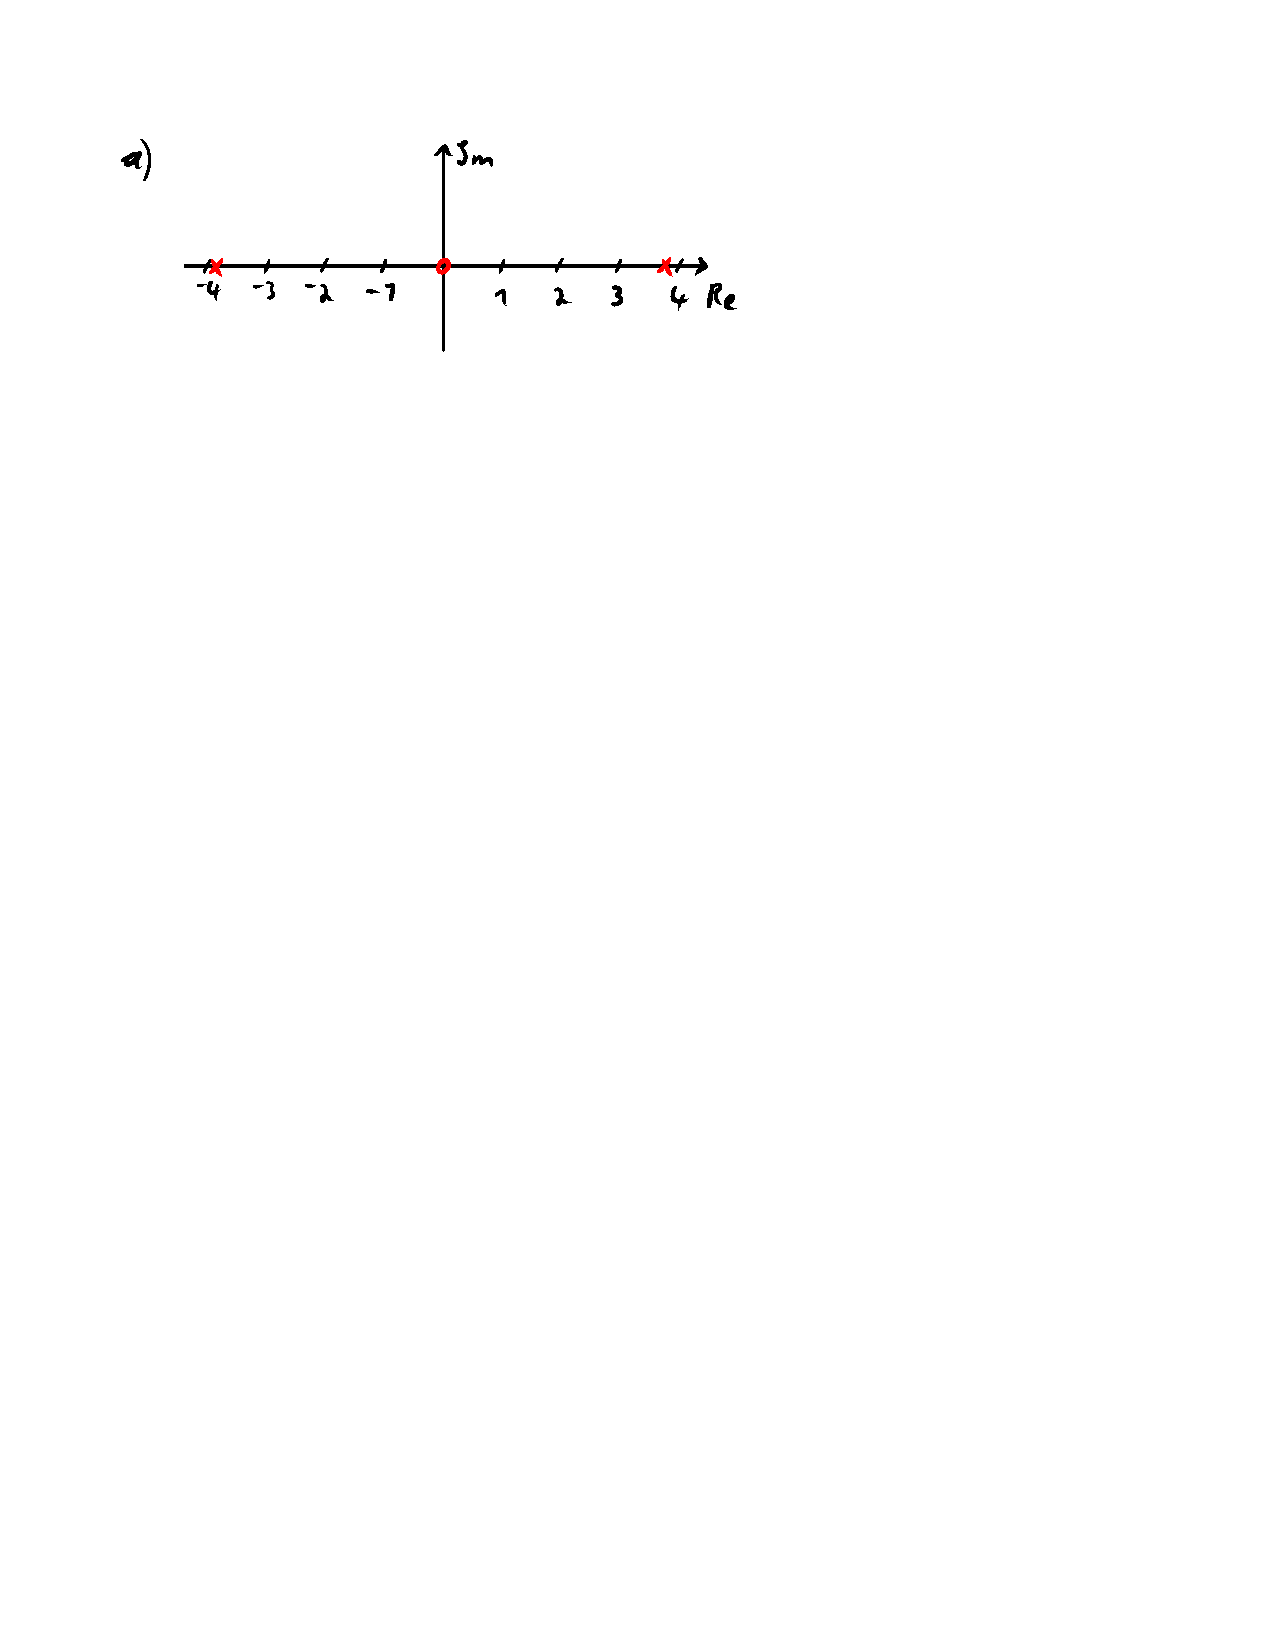
\includegraphics[scale=1, trim = 3cm 21.5cm 9cm 2cm, clip]{Bilder/Polnullstellen_G}
                \caption{Polnullstellendiagramm der Strecke}
                \label{fig:Polnullstellen_G}
        \end{figure}
         \\ %scale=1, trim = 2cm 21.5cm 9cm 2cm, clip     
        
	\end{quote} %Ende Subsection Linearisierung
	
	\subsection{Wurzelortskurve}
    Aufgabe:\\
    Machen Sie sich mit den Konstruktionsregeln für Wurzelortskurven vertraut! Gegeben sei der folgende Regler\\
    \begin{equation*}
        \begin{split}
            G_r(s) = K\frac{s + \alpha}{s + \beta}, \ \ K,\alpha, \beta \in  \Re
        \end{split}
    \end{equation*}
    mit $K > 0$. Entscheiden Sie anhand des Wurzelortskurvenverfahrens über die notwendige Lage der Reglerpolstelle
    und -nullstelle, damit das geregelte System für eine genügend große Verstärkung $K$ stabilisiert werden kann.
    Bestimmen Sie nur, in welcher Hälfte der s-Ebene jeweils die Pol- und die Nullstelle liegen muss und nicht die
    genaue Position.\vspace{1em}
    
    \begin{quote}
        
        
        Um herauszufinden wo die Pol- und Nullstelle des Reglers liegen müssen, Skizzieren wir zunächst alle vier Möglichkeiten.
        
        
        \begin{figure}[H]
        \centering
            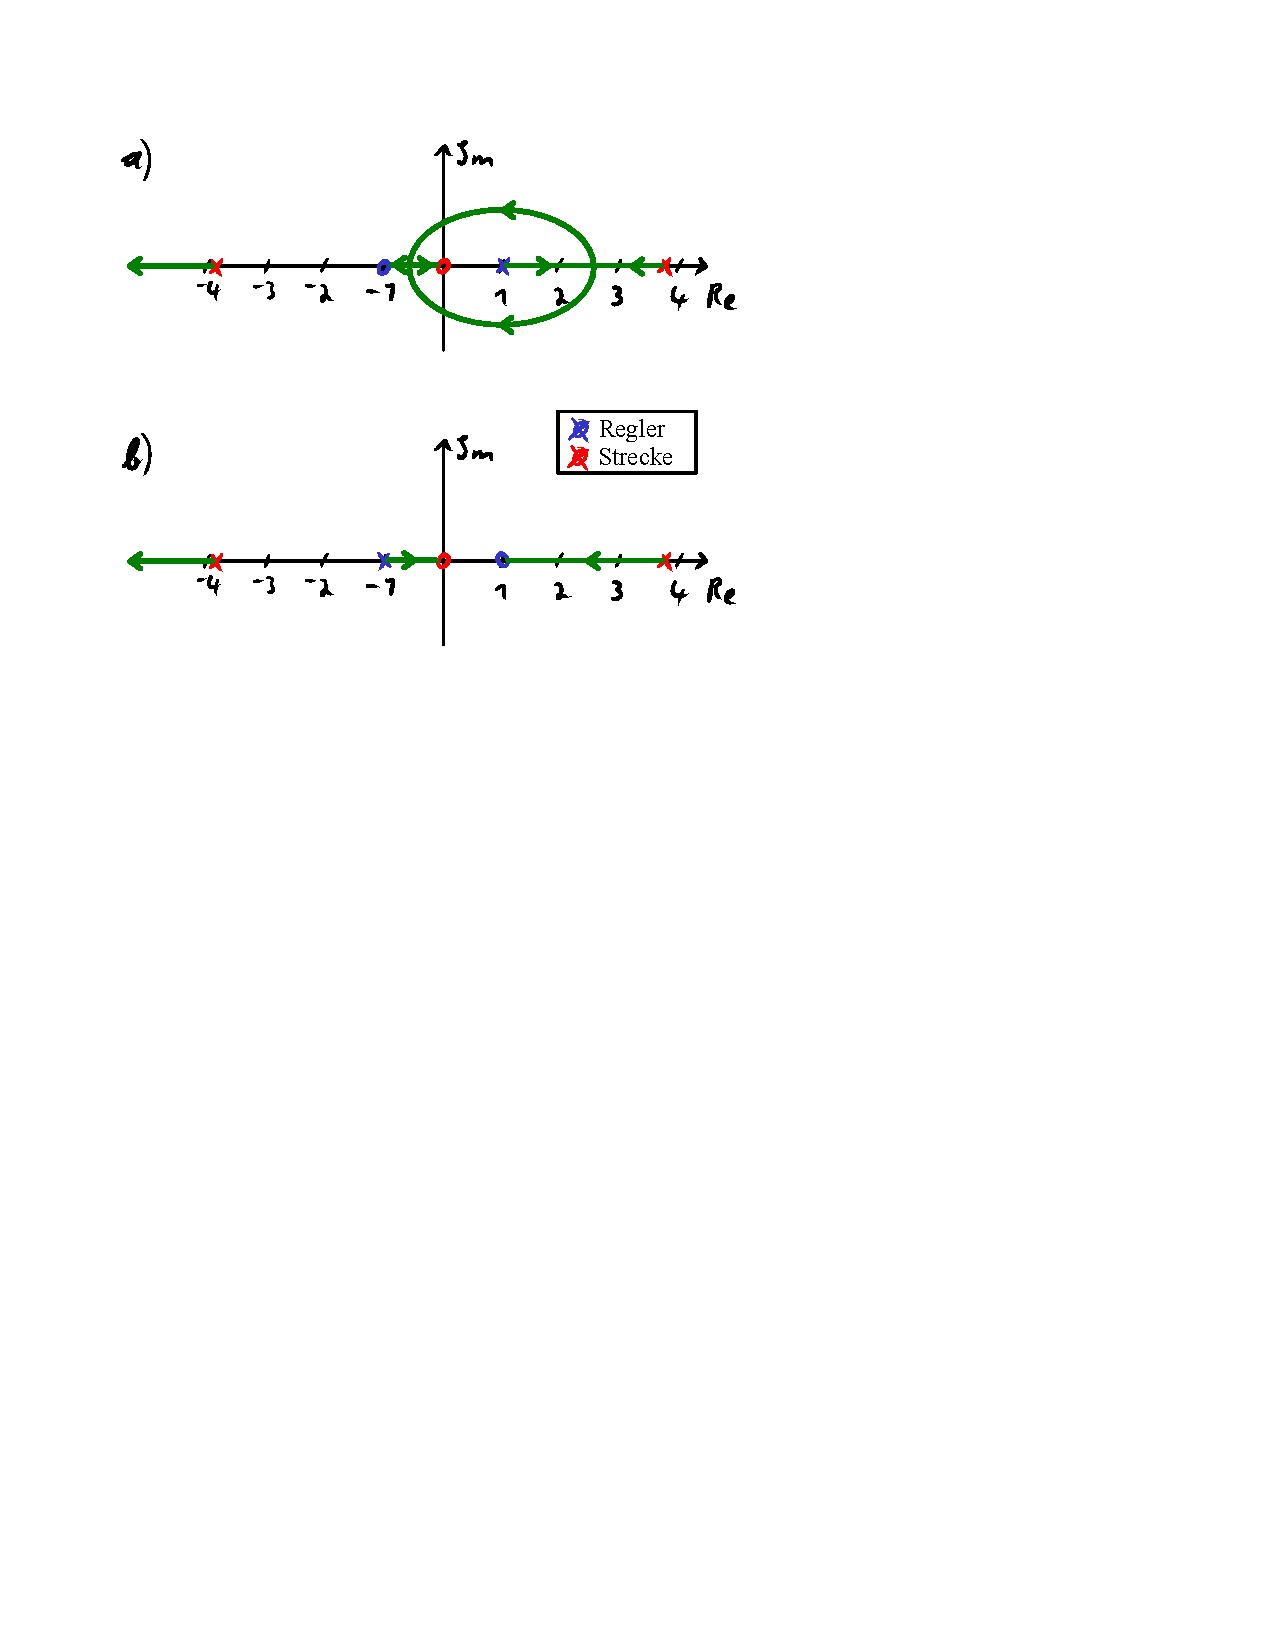
\includegraphics[scale=1, trim = 2cm 16.7cm 9cm 2cm, clip]{Bilder/WOK_GK_phi}
                \caption{WOK: a)\ $\alpha > 0,\ \beta < 0$; \ \ b) $\alpha < 0,\ \beta > 0$}
                \label{fig:WOK_GK_phi}
        \end{figure}
        
        Die Wurzelortskurve \ref{fig:WOK_GK_phi}a) mit $\alpha > 0,\ \beta < 0$ zeigt, dass bei genügend hoher Verstärkung die
        beiden instabilen Pole in die linke Halbebene wandern und der geschlossene Regelkreis somit stabil wäre. Daher wär diese
        Wahl der Pol-/Nullstellen möglich.\\
        \\
        An der Skizze \ref{fig:WOK_GK_phi}b) kann man hingegen sehen, dass die Polstelle der Strecke auch für unendlich hohe
        Verstärkung in der positiven Halbebene bleibt.
        
        
        \begin{figure}[H]
        \centering
            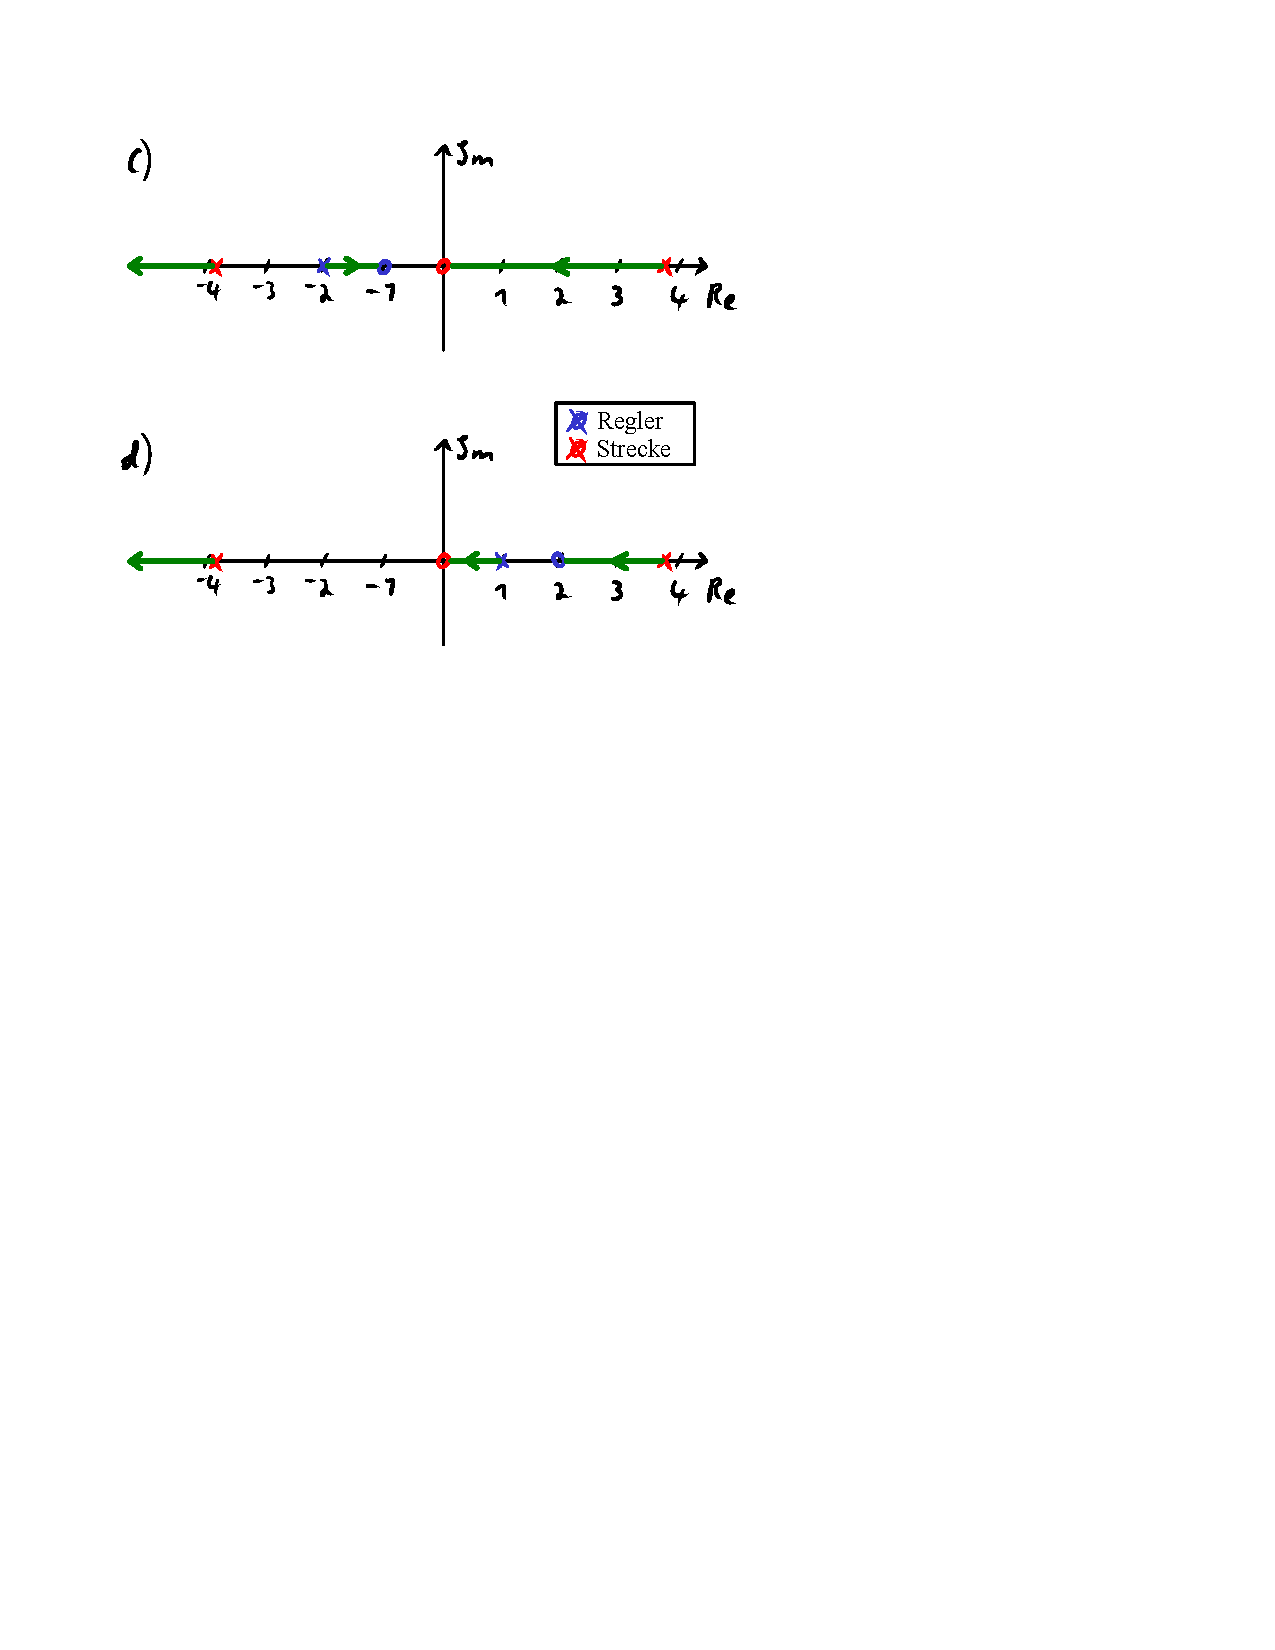
\includegraphics[scale=1, trim = 2cm 16.7cm 9cm 2cm, clip]{Bilder/WOK_GK_phi_2}
                \caption{WOK: c)\ $\alpha > 0,\ \beta > 0$; \ d) $\alpha < 0,\ \beta < 0$}
                \label{fig:WOK_GK_phi_2}
        \end{figure}
        
        
        Die Grafik \ref{fig:WOK_GK_phi_2}c) lässt erkennen, dass die unstabile Polstelle der Strecke erst für eine Verstärkung von
        unendlich im Uhrsprung ist und das System dan auch nur Stabil und nicht asymptotisch Stabil wäre.\\
        \\
        Die Skizze \ref{fig:WOK_GK_phi_2}d) zeigt wieder, dass diese Plazierung der Pole und Nullstellen des Reglers zu einem
        instabielen Regelkreis führen würde, da die positive Polstelle der Strecke in der rechten Halbbene, und somit Instabil
        bleibt.\\
        \\
        \\
        Da wir die drei letzten Varianten ausschließen könnten bleibt uns nur $\alpha > 0,\ \beta < 0$ zu wählen. Nur bei dieser
        Anordnung der Pol-/Nullstellen des Reglers wandern alle instabilen Pole bei endlicher Verstärkung in die negative
        Halbebene und der geschlossene Regelkreis wird somit Stabil.
        
        
	\end{quote} %Ende Subsection WOK
	
	\subsection{Nyquistkriterium}
	Aufgabe:\\
    Machen Sie sich mit dem allgemeinen Nyquistkriterium vertraut! Skizzieren Sie mit der zuvor bestimmten
    Pol-/Nullstellenverteilung des Reglers das Nyquistdiagramm des offenen Regelkreises. Gegebenenfalls kann eine
    konkrete Realisierung des Reglers angenommen werden, um das Nyquistdiagramm zeichnen zu können. Welche Bedingungen
    werden nach dem Nyquistkriterium an die Ortskurve der offenen Kette hinsichtlich der Stabilität gestellt und wie
    kann man dieses Bedingungen im Bodediagramm wiederfinden?\vspace{1em}
    
    \begin{quote} 
   
    \begin{figure}[H]
        \centering
            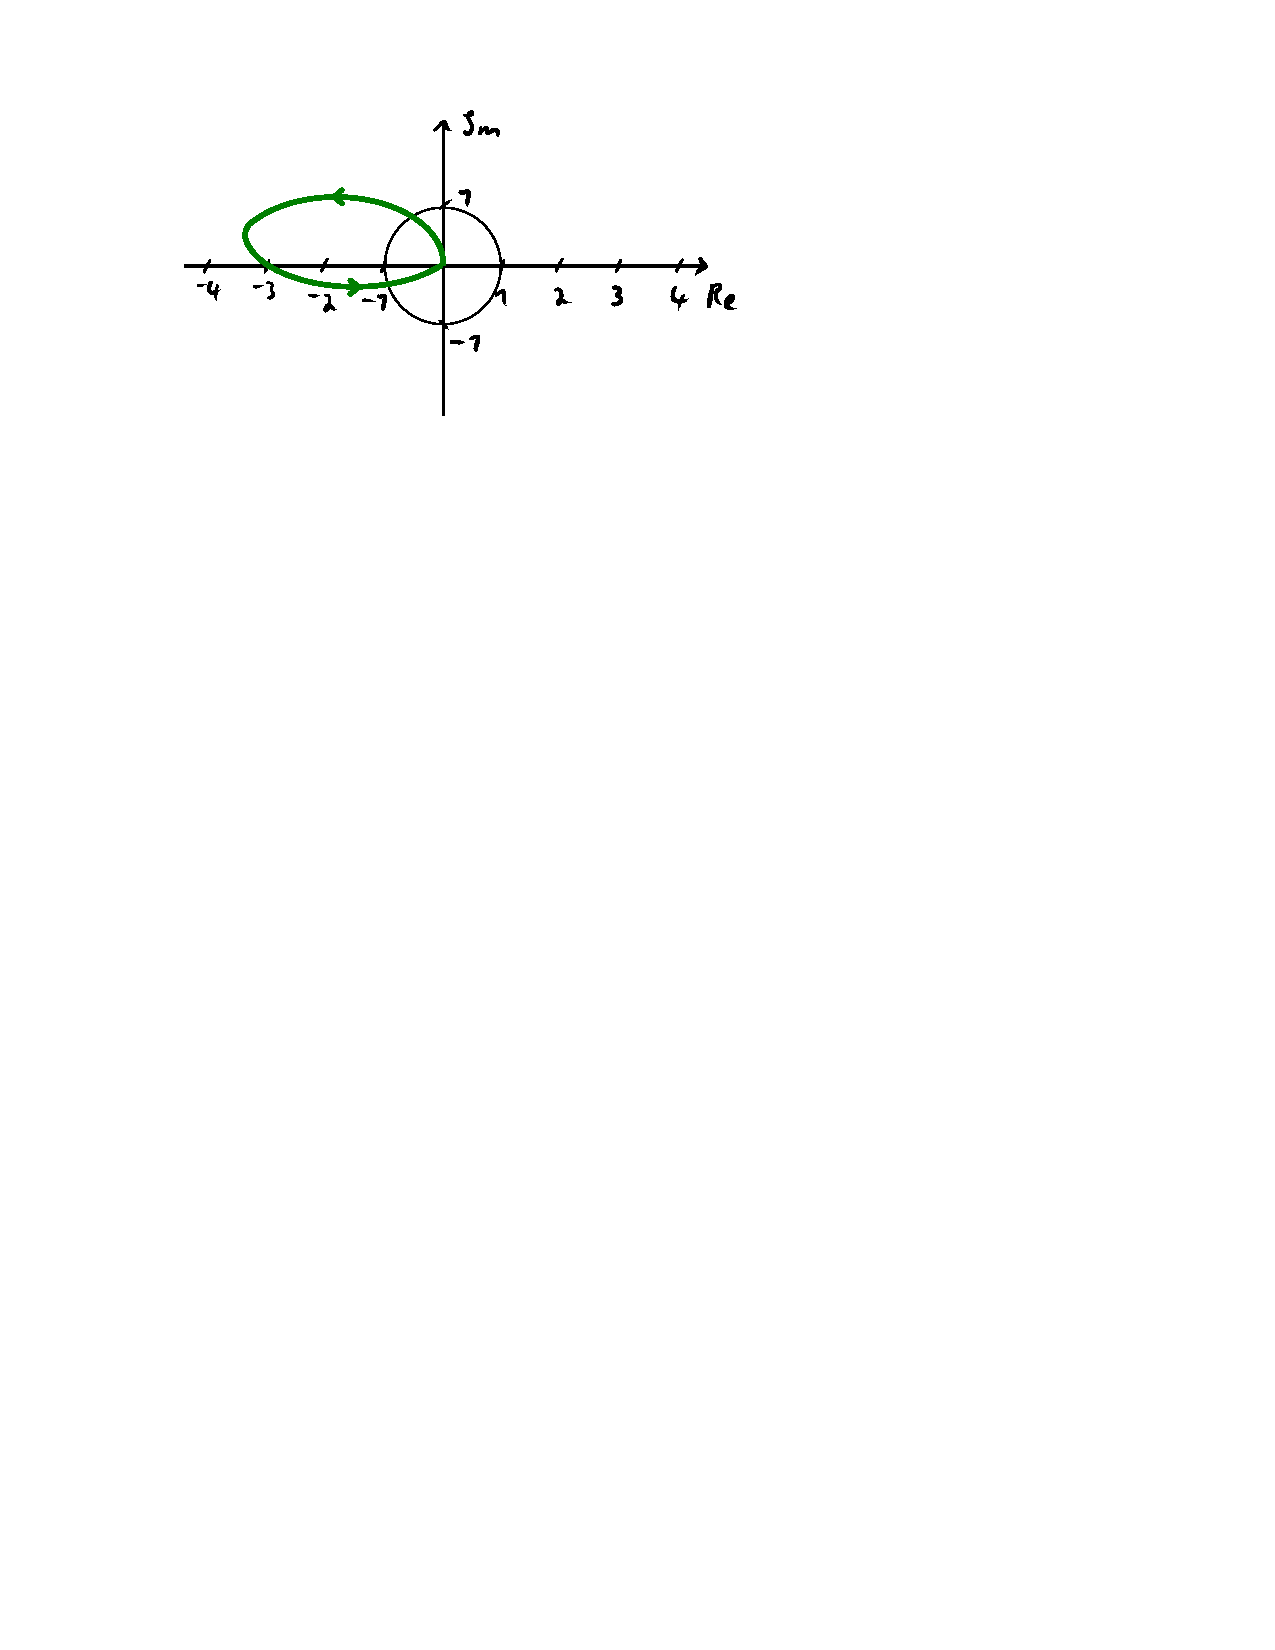
\includegraphics[scale=1, trim = 3cm 21.5cm 9cm 1.5cm, clip]{Bilder/Nyquist_kurve}
                \caption{Nyquistkurve}
                \label{fig:Nyquist_kurve}
        \end{figure}
        
        Anhand der Nyquistortskurve lässt sich die Stabilität eines geschlossenen Regelkreises für eine feste
        Verstärkung ermitteln. Dazu darf die Nyquistortskurve nicht durch den kritischen Punkt ($-1,0$) laufen und
        die Phasendrehung bezüglich des kritischen Punktes muss genau $\pi \cdot (r_G + r_K)$ betragen.\\
        $r_G$ und $r_K$ sind in diesem Fall die Anzahl der Polstellen mit positiven Realteil der Strecke bzw. des
        Reglers.
        Außerdem lassen wir die Nyquistorstkurve von $0$ bis $\infty$ laufen. Würden wir sie von $-\infty$ bis $\infty$
        laufen lassen, müsste die Phasendrehung $2\pi (r_G + r_K)$ sein.\vspace{1em}
        
        In unserem Fall haben wir eine Polstelle mit positivem Realteil in der Strecke und eine Polstelle im Regler. Daher
        benötigen wir eine Nyquistortskurve die nicht durch den kritischen Punkt läuft und eine Phasendrehung von $2\pi$ hat um
        ein stabilen geschlossenen Regelkreis zu haben.\\
        Diese Bedingung prüfen wir beim Reglerentwurf im nächsten Aufgabenabschnitt.\vspace{1em}
        
        \begin{figure}[H]
        \centering
            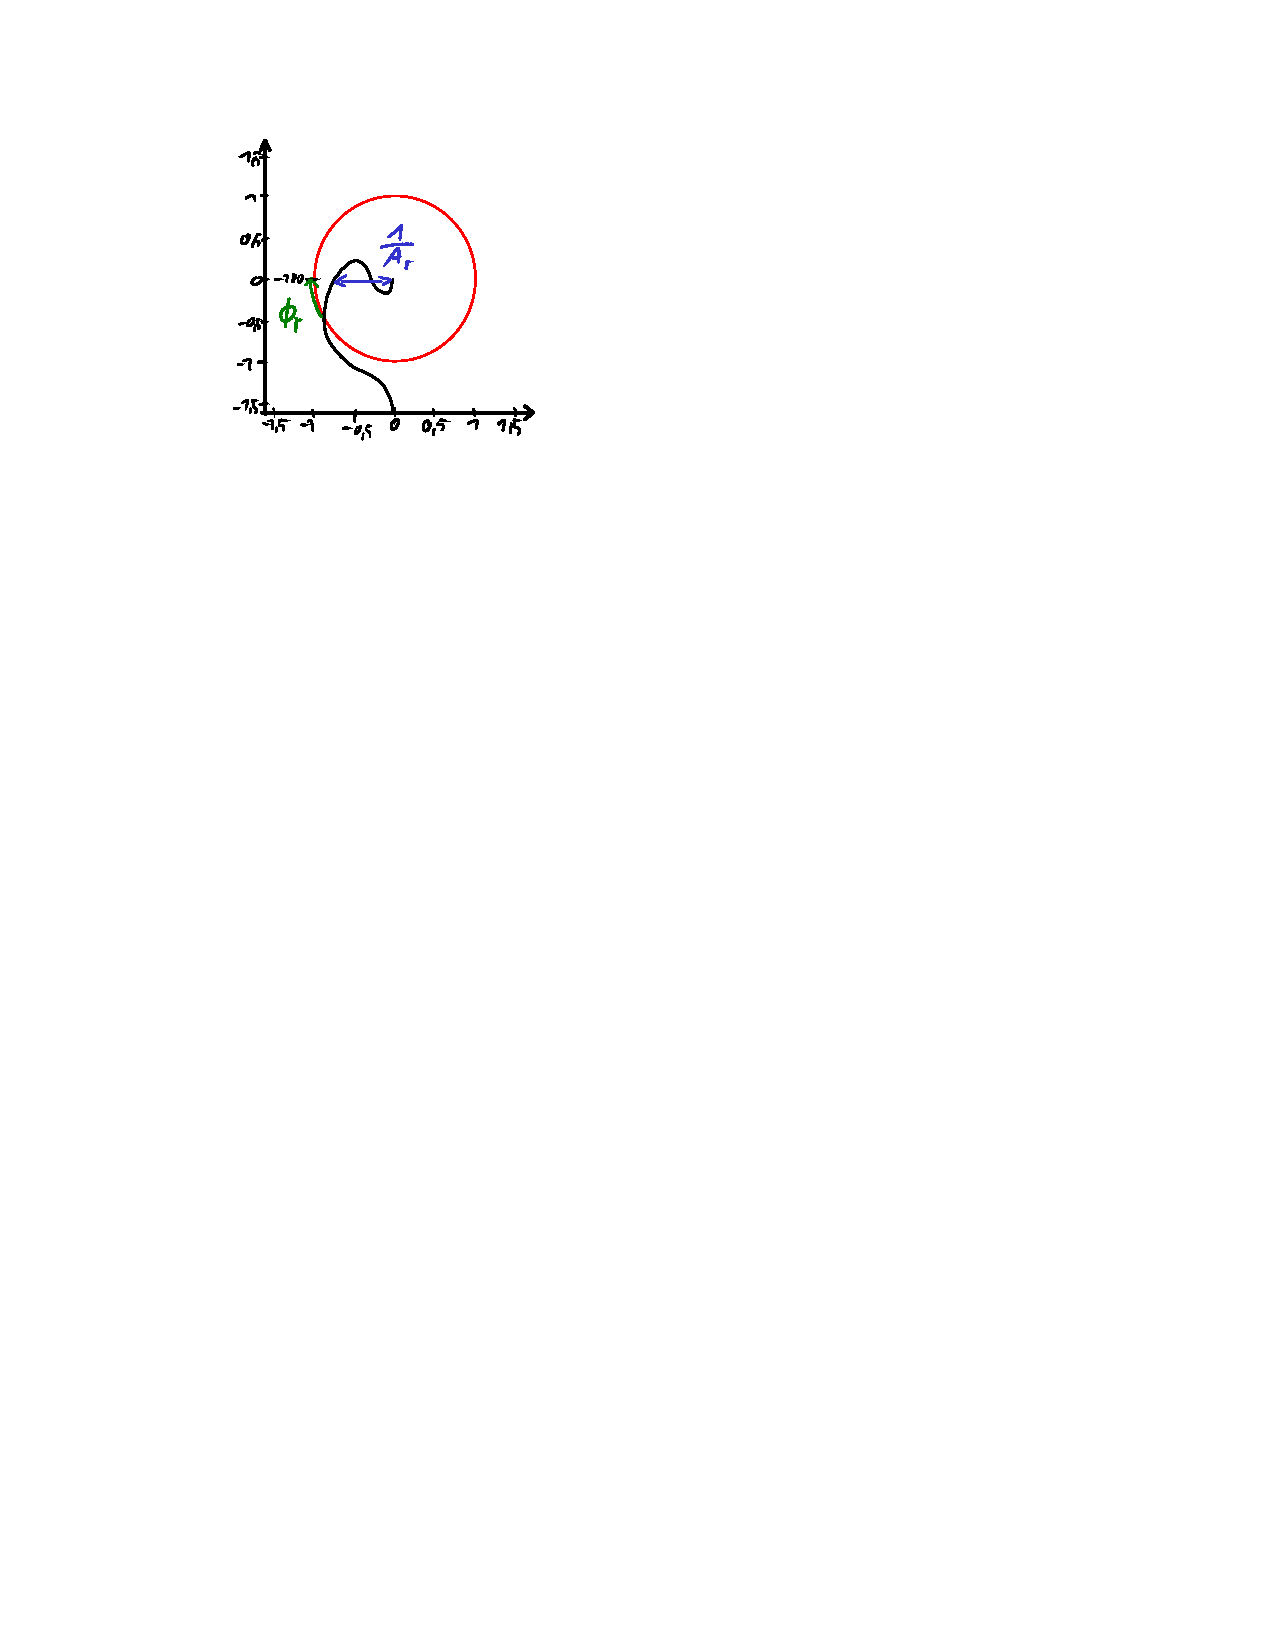
\includegraphics[scale=1.3, trim = 4cm 20.5cm 12.5cm 2cm, clip]{Bilder/Nyquist_beispiel}
                \caption{Beispielhafte Nyquistkurve mit Amplituden- und Phasenreserve}
                \label{fig:Nyquist_beispiel}
        \end{figure}
        
        
        Nachdem die Stabitität des geschlossenen Regelkreises bestätigt wurde, lassen sich an der Nyquistortskurve noch weitere
        Informationen, wie die Phasenreserve und die Amplitudenreserve, ablesen. Die Phasenreserve des Regelkreises erkennt
        man am Winkel zwischen dem Schnittpunkt der Nyquistortskurve mit dem Einheitskreis und der negativen reellen
        Achse. (siehe Abb. \ref{fig:Nyquist_beispiel}) Die Amplitudenreserve widerum erkennt man an dem Kehrwert des Abstandes
        zwischen der y-Achse und dem Schnittpunkt der Ortskurve mit der negativen reellen Achse.\\
        Die Phasenreserve und die Amplitudenreserve lassen sich auch an dem Bodediagramm ablesen. Hier ist die
        Phasenreserve die Differenz der Phase zu $180^{\circ}$ bei der bzw. den Durchstrittsfrequenzen. Die Amplitudenreserve
        ist die Differenz des Amplitudenganges zu $0dB$ bei der Frequenz von $180^{\circ}$.\vspace{1em}
        
        Wie oben beschrieben erwarten wir für unseren stabilen Regelkreis eine Phasendrehung von $2\pi$. Daraus resultiert
        automatisch, dass die Nyquistortskurve zweimal den Einheitskreis schneiden wird. Diese beiden Schnittpunkte mit dem
        Einheitskreis werden in dem Bodediagramm durch einen zweifache Schnittstelle mit der $0dB$ Achse im Amplitudengang zu
        sehen sein.\\
        
        
        
    \end{quote} %Ende Subsection Nyquist
    
    \subsection{Frequenzkennlinienentwurf}
    \begin{quote}
        In diesem Aufgabenteil wurden uns 5 Bedingungen gegeben die beim folgenden Reglerentwurf zu berücksichtigen
        waren. Die Erfüllung dieser Bedingungen kontrollieren wir an der Nyquistortskurve sowie dem Bodediagramm.\\
        Wir beginnen mit dem Bode-Diagramm bei einer Verstärkung von $1$. Eine der Bedingungen war es, bei einer Frequenz
        von $220 \frac{rad}{s}$ eine Dämpfung von $-42 dB$ zu erhalten. Da diese Dämpung gerade so bei der Verstärkung
        von $1$ erfüllt wird wissen wir, dass wir die Verstärkung bei $1$ belassen und für die weiteren Bedingungen die
        Position der Pol- und der Nullstelle des Reglers verändern müssen.\vspace{1em}
        
        Durch einiges Probieren setzen wir die Polstelle auf die Position $0.2$ und die Nullstelle auf die Position
        $-20$.
        
        Daraus resultiert folgende Wurzelortskurve:
        
        \begin{figure}[H]
        \centering
            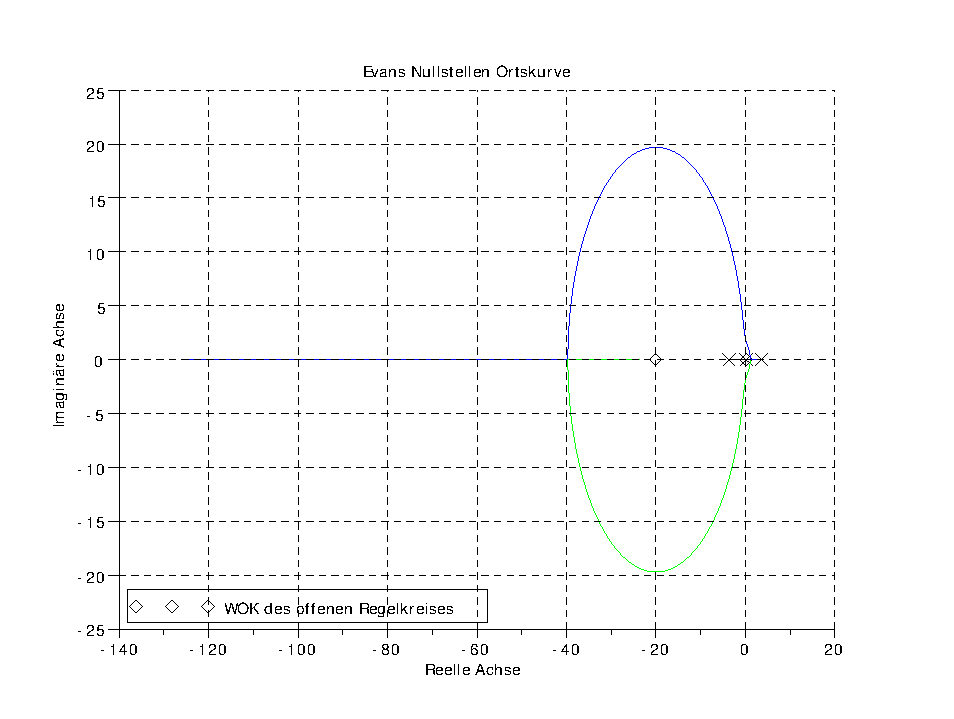
\includegraphics[scale=0.7, trim = 0cm 0cm 0cm 0cm, clip]{./Bilder/WOK}
                \caption{Wurzelortskurve}
        \end{figure}
        
        Es ist ersichtlich, dass der geschlossene Regelkreis für eine genügend große Verstärkung stabil
        wird.\vspace{1em}
        
        Außerdem ergibt sich auch folgende Nyquistkurve:
        
        \begin{figure}[H]
        \centering
            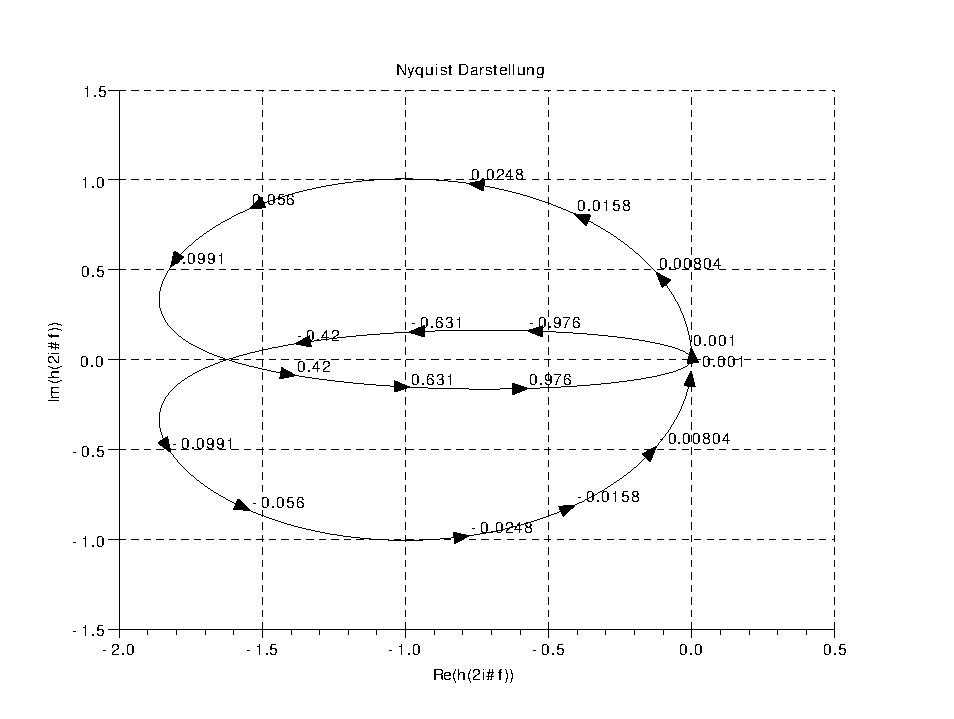
\includegraphics[scale=0.7, trim = 0cm 0cm 0cm 0cm, clip]{./Bilder/Nyquistkurve}
                \caption{Nyquistkurve}
        \end{figure}
        
        Da Scilab die Nyquistkurve von $-\infty$ bis $\infty$ berechnet, benötigen wir eine Phasendrehung von $4\pi$ um ein
        stabiles System zu erstellen. Diese Bedingung ist offensichtlich erfüllt.\vspace{1em}
        Aus den Werten ergibt sich das folgende Bodediagramm:
        
        \begin{figure}[H]
        \centering
            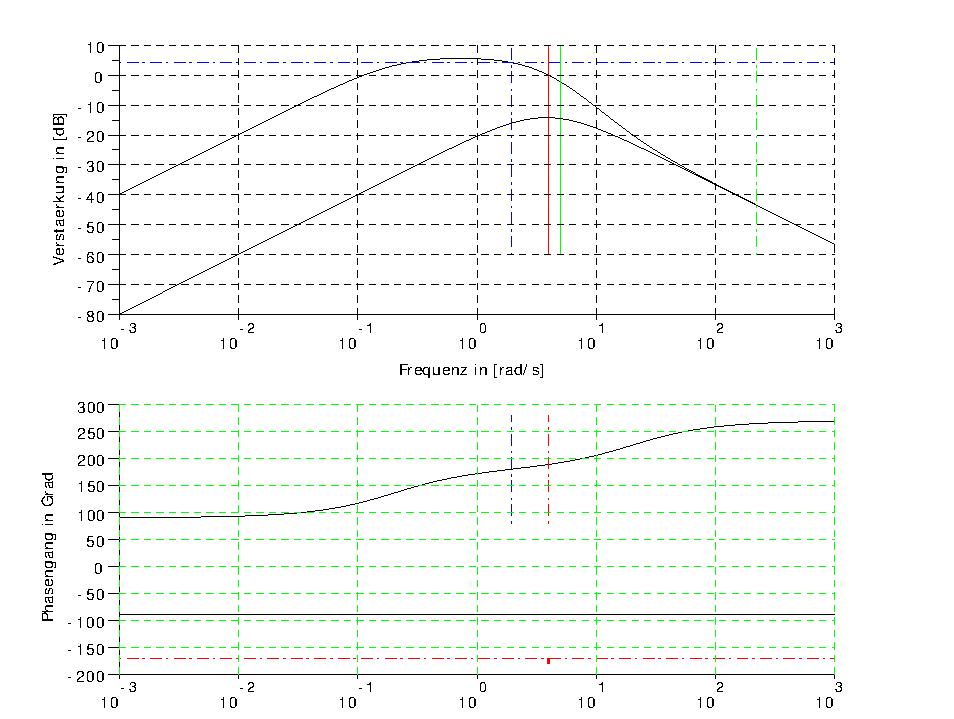
\includegraphics[scale=0.7, trim = 0cm 0cm 0cm 0cm, clip]{./Bilder/Bodediagramm}
                \caption{Bodediagramm}
        \end{figure}
        
        Die Amplitudenreserve beträgt: $-4.2035059 dB$ und die Phasenreserve $8.8051927 ^{\circ}$. Für alle Frequenzen
        größer als $4\frac{rad}{s}$ ist der Amplitudengang kleiner als $0dB$. Außerdem ist die Dämpfung bei der Frequenz
        $220 \frac{rad}{s}$ ca. $-43.3 dB$. Somit sind alle Vorgaben erfüllt. 
    
    \end{quote}  % Ende Subsection Frequenzkennlinienentwurf
    
    \subsection{Führungsverhalten}
    \label{sec:Fuehrungsverhalten}
    
    Aufgabe\\
    Untersuchen Sie das Verhalten des Regelkreises gegenüber konstanten Sollvorgaben ungleich Null. Wie verhalten sich
    Wagenposition, Winkel und Wagengeschwindigkeit?\vspace{1em}
    
    \begin{quote}
        In diesem Aufgabenteil haben wir das Verhalten des bisherigen Regelkreises auf einen Führungssprung untersucht.
        Dazu haben wir das nichtlineare Modell in Xcos implementiert und das Sprungverhalten simuliert und untersucht. Leider hat
        sich herausgestellt, dass das von uns erstellte nichtlineare Modell der Strecke fehlerhaft ist und nicht das erwarteten
        Verhalten zeigt. Selbst nach langem Suchen und der Hilfe unseres Tutors haben wir den Fehler nicht finden können. Daher
        erstellen wir die in diesem Versuch benutzten Plots mit dem nichtlinearen Modell unseres Tutors.\vspace{1em}
        
        
        Um die Führungssprungantwort dieses Regelkreises zu bestimmen geben wir einen Sprung auf die Führungsgröße des
        Winkelreglers. Der Regler ist ausgelegt auf ein Einzugsbereich von einigen Grad. Da die Führungsgröße jedoch in
        $rad$ gemessen wird wäre ein Sprung auf $1 rad$ bzw. $1\cdot \frac{180}{\pi} ^{\circ}= 57.29578^{\circ}$ viel zu
        groß für den Regler. Daher geben wir einen Sprung von $0$ auf $2^{\circ} = 0.0349066 rad$ auf die
        Führungsgröße.\vspace{1em}
        
        Zuerst schauen wir uns die Antwort des Winkels auf diesen Sprung an.
        
        \begin{figure}[H]
        \centering
            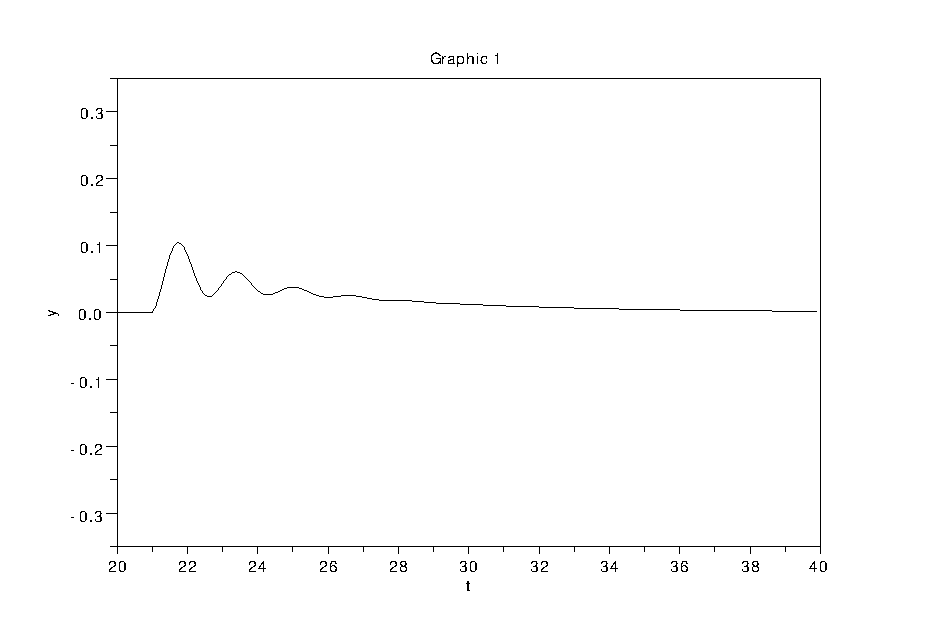
\includegraphics[scale=0.7, trim = 0cm 0cm 0cm 0cm, clip]{./Bilder/Winkelregler_Winkel}
                \caption{Winkelregler Winkel}
        \end{figure}
        
        Es ist zu sehen, dass der Regeler den Winkel nicht wie bei den bisher behandelten Reglern auf die Führungsgröße
        hochregelt, sondern den Winkel sofort auf $0^{\circ}$ zurückregelt. Da wir versuchen das Pendel in seiner
        instabilen Ruhelage von $0^{\circ}$ zu halten ist dieses Verhalten gewünscht.\vspace{1em}
        
        Als nächstes betrachten wir die Wagengeschwindigkeit.
        
        \begin{figure}[H]
        \centering
            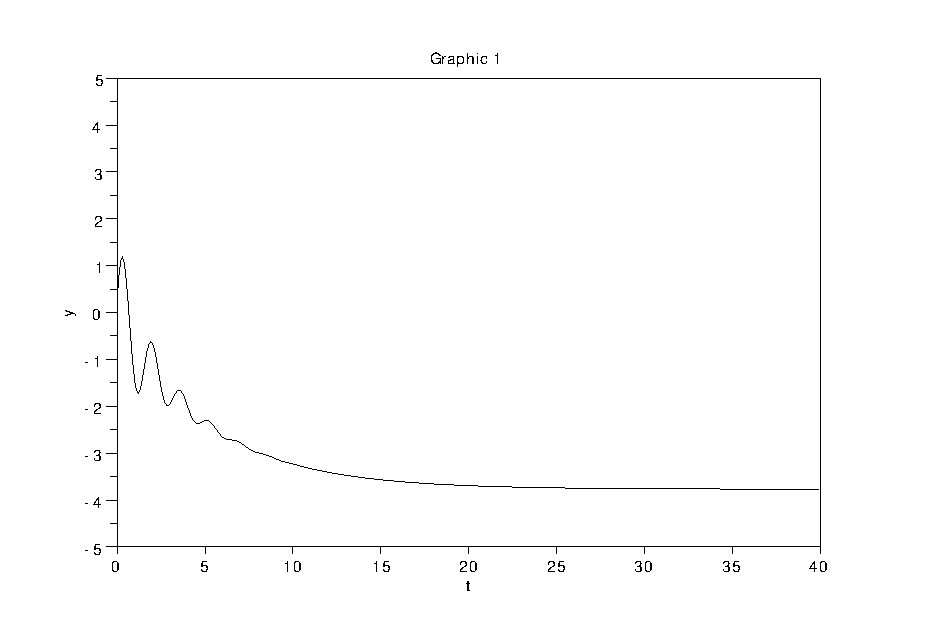
\includegraphics[scale=0.7, trim = 0cm 0cm 0cm 0cm, clip]{./Bilder/Winkelregler_Wagengeschwindigkeit}
                \caption{Winkelregler Wagengeschwindigkeit}
        \end{figure}
        
        Es ist zu beobachten, dass der Wagen am Anfang des Ausregelvorgangs zügig seine Geschwindigkeit ändert. Interessant
        ist, dass er gegen Ende des Ausregelvorgangs bei einer konstanten Geschwindigkeit $\neq 0$ angekommen ist und
        auf dieser bleibt. Die Ursache dafür ist, dass unser Regler zu diesem Zeitpunkt lediglich das Ziel hat auf eine
        Winkelposition von $0^{\circ}$ zu regeln. Die Position des Wagens wird noch nicht berücksichtigt. Daher ist es
        für den Regler vollkommen ausreichend das Pendel unter konstanter Gesamtgeschwingigkeit des Systems bei der
        gewünschten Winkelposition zu belassen.\\
        Der Regler bremst den Wagen nicht wieder ab, da das Pendel durch die Massenträgheit sofort wieder kippen würde.
        \vspace{1em}
        
        Als letztes betrachten wir die Position des Wagens.

        \begin{figure}[H]
        \centering
            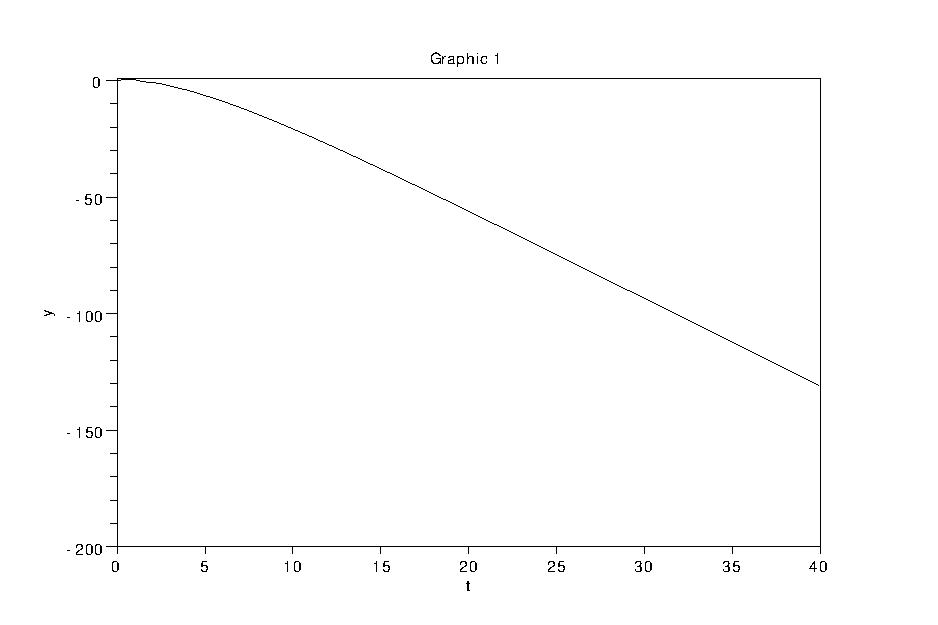
\includegraphics[scale=0.7, trim = 0cm 0cm 0cm 0cm, clip]{./Bilder/Winkelregler_Position}
                \caption{Winkelregler Position}
                \label{Winkelregler_Position}
        \end{figure}
        
        Da wir bei der Wagengeschwindigkeit herausgefunden haben, dass der Regler bei einer konstanten Geschwindigkeit
        bleiben wird, ist es nur logisch, dass der Wagen sich dadurch immer weiter vom Ursprung entfernt.
        Genau dieses Verhalten ist in der Grafik zu sehen. Theoretisch haben wir somit einen funktionstüchtigen Regler
        entworfen, jedoch zeigt diese Grafik auch die Schwierigkeit des bisherigen Entwurfs. Dieser Regler würde unendlich
        viel Platz benötigen. Um diese Problematik in den Griff zu bekommen werden wir noch einen äußeren Regler für die
        Positionsregelung entwerfen.
        
        
    \end{quote}  % Ende Subsection Führungsverhalten
    
    \subsection{Störverhalten}
    Aufgabe\\
    Untersuchen Sie das Verhalten des Regelkreises bei konstanten Ausgangsstörungen (z.B. durch Messfehler oder Wagen
    auf geneigter Ebene). Wie verhalten sich Wagenposition, Winkel und Wagengeschwindigkeit?\vspace{1em}
    
    \begin{quote}
        Um die Störsprungantworten mit den Führungssprungantworten vergleichbar zu machen geben wir den selben Sprung auf das
        System. Jedoch nicht als Führungsgröße sondern als Störung am Ausgang des Systems. Eine konstante Ausgangsstörung
        unterscheidet sich in diesem Fall lediglich in dem Vorzeichen von einem Führungssprung. Aus diesem Grund erwarten wir die
        selben Sprungantworten.
        
        \begin{figure}[H]
        \centering
            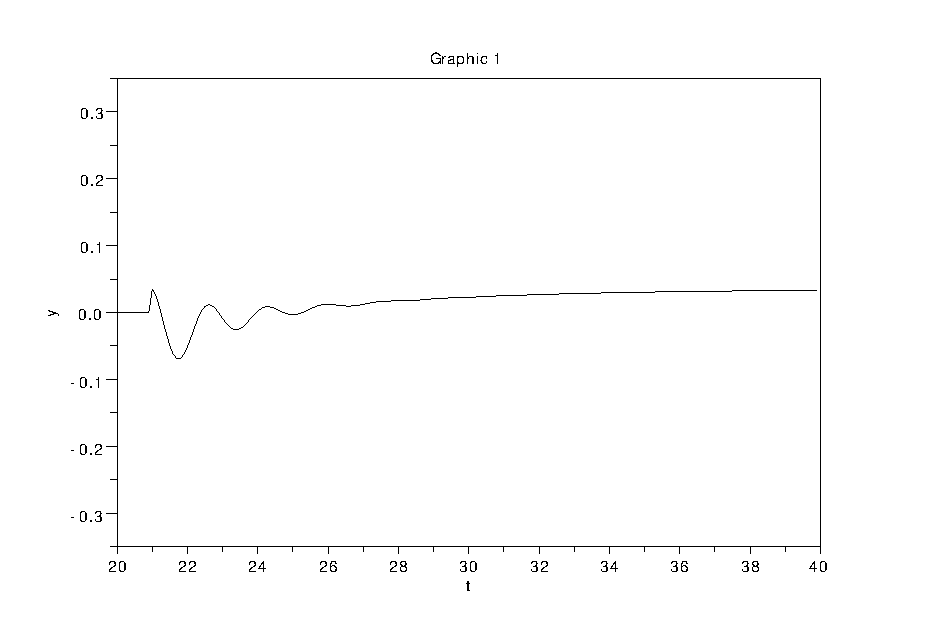
\includegraphics[scale=0.7, trim = 0cm 0cm 0cm 0cm, clip]{./Bilder/Winkelregler_Stoer_Winkel}
                \caption{Winkelregler Störspungantwort Winkel}
        \end{figure}
        
        \begin{figure}[H]
        \centering
            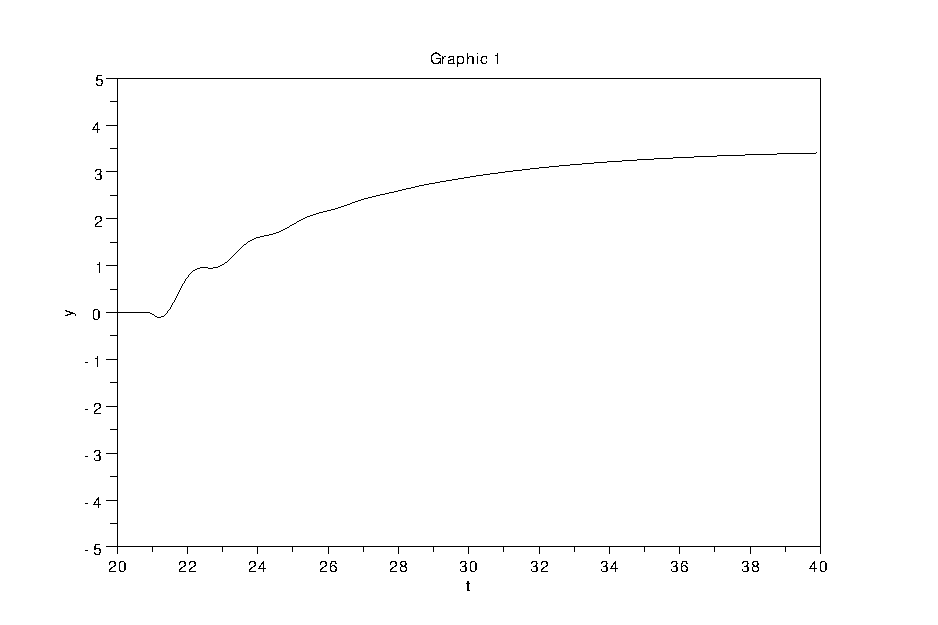
\includegraphics[scale=0.7, trim = 0cm 0cm 0cm 0cm, clip]{./Bilder/Winkelregler_Stoer_Wagengeschwindigkeit}
                \caption{Winkelregler Störsprung Wagengeschwindigkeit}
        \end{figure}  
        
        \begin{figure}[H]
        \centering
            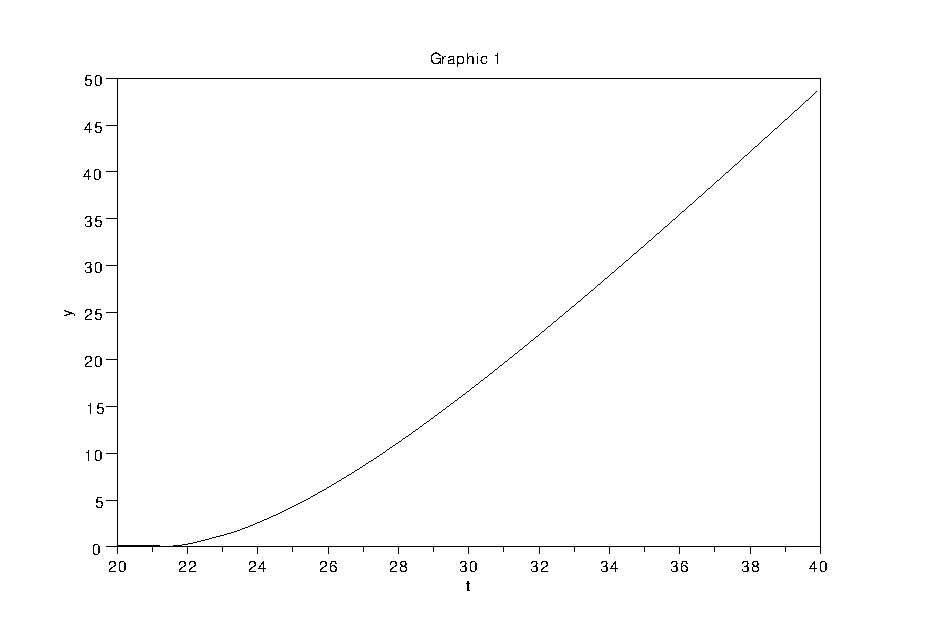
\includegraphics[scale=0.7, trim = 0cm 0cm 0cm 0cm, clip]{./Bilder/Winkelregler_Stoer_Position}
                \caption{Winkelregler Störsprung Position}
        \end{figure}
        
        
        Die Störsprungantworten verhalten sich genau wie die Führungssprungantworten und damit genauso wie wir es
        erwartet haben.
        
    \end{quote}  % Ende Subsection Störverhalten
    \vspace{1em}
    
    \textbf{Von hier an ergänzen wir das System mit einem Positionsregler}.
    
    
    \subsection{Übertragungsverhalten des inneren Kreises}
    Aufgabe:\\
    Bestimmen Sie das linearisierte Übertragungsverhalten des inneren Regelkreises am Arbeitspunkt ($\varphi, z$) =
    ($0, 0$) mit dem Regler $G_r(s)$ aus dem Versuch 1a. Gesucht ist die Transferfunktion vom Sollwinkel $\varphi_r$ auf
    die Wagenpositions $z$.\\
    Welche Ordnung hat der geschlossene innere Regelkreis?\vspace{1em}
    
    \begin{quote}
        Die Transferfunktion vom Sollwinkel zur Wagenposition lässt sich sehr gut am Blockschaltbild des Reglers ablesen. 
        
        \begin{figure}[H]
        \centering
            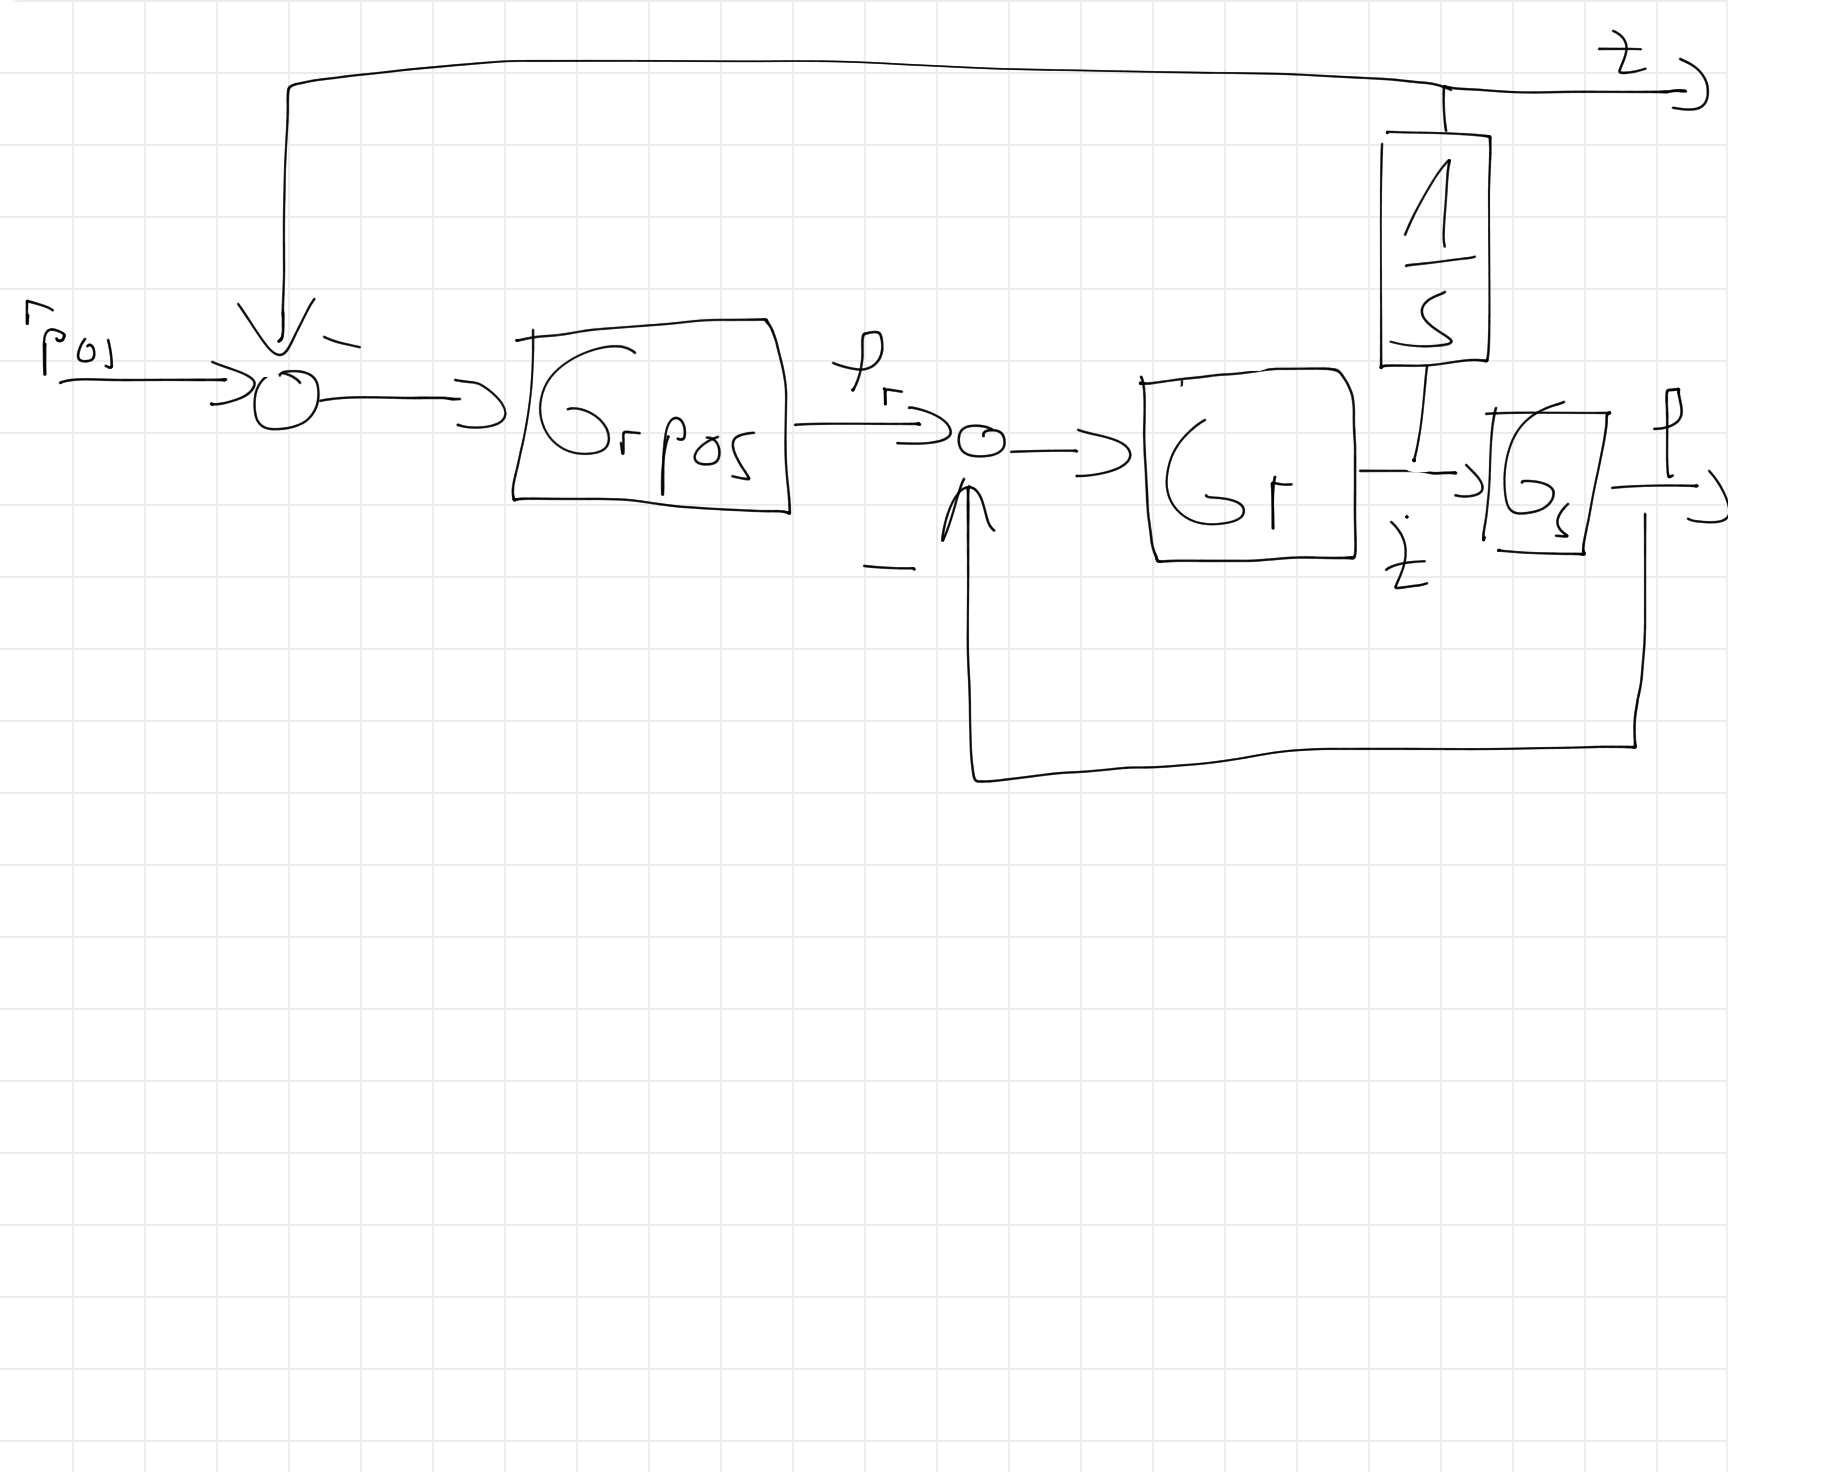
\includegraphics[scale=0.3, trim = 0cm 12cm 0cm 0cm, clip]{./Bilder/Blockschaltbild}
                \caption{Blockschaltbild}
        \end{figure}
    
        Hieraus ergibt sich die Transferfunktion:

        \begin{equation*}
        	\begin{split}
        		\frac{z}{\varphi_r} = \frac{G_r \frac{1}{s}}{1 + G_r G_s}
        	\end{split}
        \end{equation*}
        
        Als zweite Möglichkeit lässt sich die Transferfunktion auch aus den Formeln herleiten.

        \begin{equation*}
            \begin{split}
                z &= \frac{1}{s} \dot{z}\\
                z &= G_r e\\
                e &= \varphi_r - \varphi\\
                \varphi &= G_s \dot{z}\\
                \\
                \Rightarrow z &= \frac{1}{s} \G_r e = \frac{1}{s} G_r (\varphi_r -\varphi)\\
                &= \frac{1}{s} G_r(\varphi_r - G_s \dot{z})\\
                &= \frac{1}{s} G_r(\varphi_r - G_s s z)\\
                &= \frac{1}{s} G_r \varphi_r - \frac{1}{s} G_r G_s s z\\
                z(1+G_r G_s) &= \frac{1}{s}G_r \varphi_r\\
                \frac{z}{\varphi_r} &= \frac{\frac{1}{s}G_r}{1 + G_r G_s}\\
            \end{split}
        \end{equation*}
        
        Wenn wir die besherigen Übertragungsfunktionen einsetzen ergibt sich die folgene Übertragungsfunktion des
        inneren Reglers:
        
        \begin{equation*}
        	\begin{split}
        		G_{innen} = \frac{- 291.89357 - 13.28885s + 20.065291s^2 + s^3 }{2.9189357s + 15.146959s^2 + 1.3530262s^3 +
        		s^4 }
        	\end{split}
        \end{equation*}
        
        Der geschlossene innere Regelkreis hat demnach die Ordnung $4$.
        
    \end{quote}  % Ende Subsection Übertragungsverhalten
    
    \subsection{Polvorgabe mit und ohne Reglerintegrator}
    Aufgabe:\\
    Entwerfen Sie einen Regler $G_{rPOS}$ mittels Polvorgabe für den äußeren Regelkreis mit und ohne Reglerintegrator!
    Führen Sie keine Pol-/Nullstellen-Kürzungen beim Reglerentwurf durch! Schreiben Sie eine Scilab-Routine zur
    Bestimmung der Reglerpolynome. Verwenden Sie hier für die Sylvestermatrix.\vspace{1em}
    
    Wie wirken sich Ausgangsstörungen des inneren Regelkreises auf die stationäre Genauigkeit des äußeren Kreises bei
    den beiden Reglern aus?\vspace{1em}
    
    \begin{quote}
        
        Als Vorgabe haben wir bekommen, dass das Führungsverhalten des äußeren Regelkreises dem eines dominierenden komplexen
        Polpaars entsprechen soll deren Standardübertragungsfunktion (2. Ordnung) eine ungefähre Anstiegszeit von $tr =$
        \SI{4}{\second} und eine Dämpfung von $D =$ \SI{0,97}{} besitzt.\\
        Um das Polpaar zu erhalten haben wir die vorgaben in die Übertragungsfunktion eingesetzt:
        
        
        \begin{equation*}
            \begin{split}
                \\
                \frac{1}{s^2 + 2 D \p w_0 \p s + w_0^2}\\
                \\
                w_0 = \frac{1}{t_r} e^{ \frac{D}{\sqrt{1-D^2}} \p \arccos(D) }\\
                \\
            \end{split}
        \end{equation*}
        
        daraus ergeben sich die Pole:
        
        \begin{equation}
        \begin{split}
             - 0,646013 \pm 0,1619061i
        \end{split}
        \end{equation}
        
        Da wir für unseren Regler aber 7 Pole benötigen wählen wir noch weitere Reelle Pole die schnell genug sind unser
        dominierendes Polpaar nicht zu sehr zu beeinflussen. Die Pole ergeben sich damit zu:
        
        \begin{equation*}
        \begin{split}
            - 0.646013 + 0.1619061i\\
            - 0.646013 - 0.1619061i\\
            - 8.398169\\
            - 9.398169\\
            - 10.398169\\
            - 11.398169\\
            - 12.398169\\
        \end{split}
        \end{equation*}
        
        
        Der unterschied der Regler ist, wie in Abb. \ref{fig:positionsregler_vergleich} zu erkennen nicht gravierend.
        
        \begin{figure}[H]
        \centering
            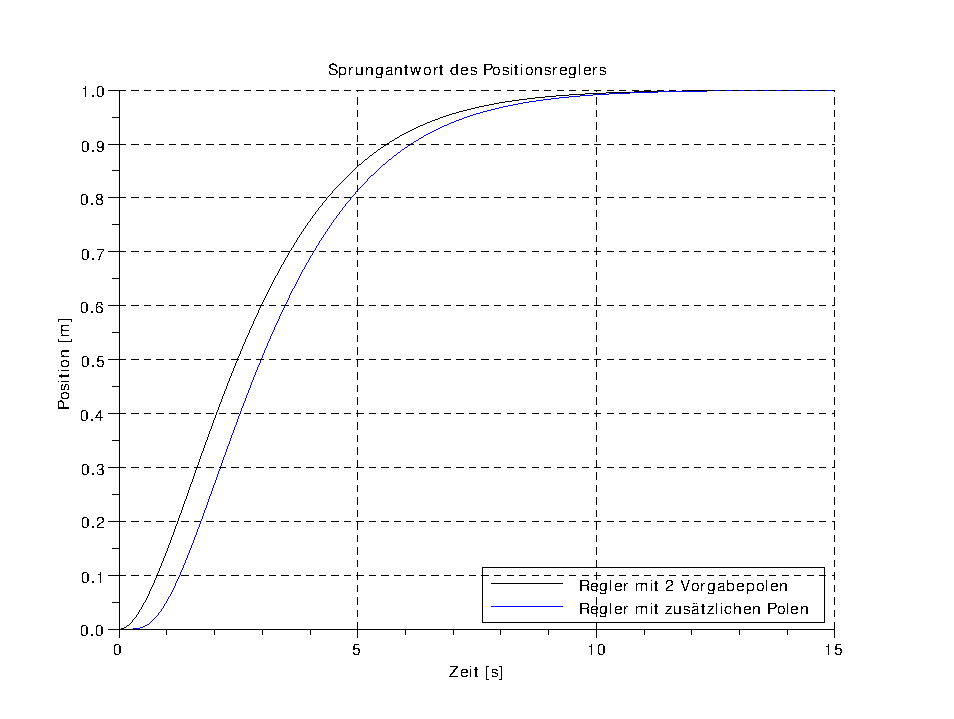
\includegraphics[scale=0.7, trim = 0cm 0cm 0cm 0cm, clip]{Bilder/positionsregler_vergleich}
                \caption{Vergleich der Sprungantworten des Positionsreglers mit 2 und 7 Polen}
                \label{fig:positionsregler_vergleich}
        \end{figure}
        
        
        Aus diesen Polen ergeben sich die Koeffizienten:
        
        
        \begin{equation*}
        \begin{split}
            51441.831\\
            175055.68\\
            194326.85\\
            71635.611\\
            12500.291\\
            1143.8363\\
            53.282871\\
            1.
        \end{split}
        \end{equation*}
        
        
        Als nächstes erstellen wir die passende Sylvestermatrix. Dazu sortieren wir die Koeffizienten der
        Übertragungsfunktion des inneren Reglers in geeineter Weise. Die Sylvestermatrix lautet:\\
        
        \begin{table}[H]
        \hspace{-4em}
        \begin{tabular}{c c c c c c c c}

            1.           &0.           &0.           &0.           &0.           &0.           &0.           &0. \\
            1.3530262    &1.           &0.           &0.           &1.           &0.           &0.           &0. \\
            15.146959    &1.3530262    &1.           &0.           &20.065291    &1.           &0.           &0. \\
            2.9189357    &15.146959    &1.3530262    &1.         &- 13.28885     &20.065291    &1.           &0. \\
            0.           &2.9189357    &15.146959    &1.3530262  &- 291.89357  &- 13.28885     &20.065291    &1. \\
            0.           &0.           &2.9189357    &15.146959    &0.         &- 291.89357  &- 13.28885     &20.065291\\
            0.           &0.           &0.           &2.9189357    &0.           &0.         &- 291.89357  &- 13.28885\\
            0.           &0.           &0.           &0.           &0.           &0.         &0.         &- 291.89357\\
        
        \end{tabular}
        \caption{Sylvestermatrix}
        \end{table} 
        \vspace{1em}
         
         Mit Hilfe der Sylvestermatrix und den Polen aus der Polvorgabe erechnen wir uns nun die Koeffizenten des
         äußeren Reglers.
         
         \begin{equation*}
        	\begin{split}
        		Reglerkoeffizienten = inv(Sylvestermatrix) \cdot Polvorgabekoeffizienten
        	\end{split}
        \end{equation*}
                
        
        Aus dieser Rechnung ergibt sich folgender Regler:
        
        \begin{equation*}
        	\begin{split}
        		K_{pos} = \frac{- 176.23489 - 500.56683s - 154.18837s^2 - 84.664893s^3 }{9113.4176 + 2796.8872s + 136.59474s^2
        		+ s^3 }
        	\end{split}
        \end{equation*}
        
        Wie wir im nächsten Aufgabenteil sehen werden, wird dieser Regler jedoch eine Regelabweichung besitzen. Diese
        können wir aber mit einem Integrator verhindern. Die Übertragungsfunktion des Reglers mit Integrator lautet
        dann:
        
        \begin{equation*}
        	\begin{split}
        		K_{PosI} &= \frac{- 33997.314 - 119043.19s - 134816.79s^2 - 27985.865s^3 - 8415.9613s^4 }{737539.64s +
        		         235184.41s^2 + 11110.757s^3 + 79.726183s^4 + s^5 }
        	\end{split}
        \end{equation*}
    \end{quote}  % Ende Subsection Polvorgabe
        
    \subsection{Darstellung von Empfindlichkeits- und komplementärer Empfindlichkeitsfunktion}
    Aufgabe:\\
    Wiederholen Sie die Begriffe Empfindlichkeits- und komplementäre Empfindlichkeitsfunktion. Was sagen diese
    Übertragungsfunktionen aus? Stellen Sie für die zuvor entworfenden Regler den Amplitudengang von Empfindlichkeits-
    und komplementärer Empfindlichkeitsfunktion dar (Betrag der Verstärkung nicht in $dB$, logarithmische Frequenz in
    $\frac{rad}{s}$).\vspace{1em}
    
    \begin{quote}
        Die Empfindlichkeitsfunktion $S$ beschreibt die Auswirkung all der Einflüsse auf die Regelgröße, die am Ausgang
        des Regelkreises auftreten. Ein Beispiel hierfür wäre eine Störung wie ein Windstoß, der das
        Pendel ein wenig zur Seite drückt. Diese Störungen sind niederfrequent. Die Funktion $S$ sollte daher eine
        starke Dämpfung im niederfrequenten Bereich aufweisen.\vspace{1em}
        
        Die komplimentäre Empfindlichskeitfunktion $T$ wiederum beschreibt die Auswirkung von den Einflüsse auf die
        Regelgröße, die am Eingang des Reglkreises auftreten. Hierfür wäre beispielhaft der Führungssprung genannt.
        Dieser ist meistens niedrigfrequent und sollte daher für niedrige Frequenzen eine konstante Verstärkung
        aufweisen. Für hohe Frequenzen, wie beispielsweise dem Rauschen sollte sie stark dämpfen.\vspace{1em}
        
        Zusätzlich gilt der Zusammenhang:
        
        \begin{equation*}
        	\begin{split}
        		S + T =1
        	\end{split}
        \end{equation*}
        
        Die beiden Funktionenen lauten:
        
        \begin{equation*}
        	\begin{split}
        		S &= \frac{- K_1 \frac{1}{s}}{1 + K_1 G_{1} + K_{pos} K_1 \frac{1}{s}}\\
        		&= -\frac{K_1}{s + K_1 G_{1} s + K_{pos} K_1}\\ \\
        		T &= \frac{K_{pos} K_1 \frac{1}{s}}{1 + K_1 G_{1} + K_{pos}K_1 \frac{1}{s}}\\
        		&= \frac{K_{pos} K_1}{s + K_1 G_{1}s + K_{pos}K_1}
        	\end{split}
        \end{equation*}

        Nachdem wir die Funktoinen $S$ und $T$ bestimmt haben überprüfen wir nun mittels Endwertsatz
        ob der Regelkreise eine bleibende Regelabweichung besitzen. Zunächst schauen wir die komplimentäre
        Sensitivitätsfunktionen $T$ an, die eine Aussage über das Verhalten des Regelkreises auf einen Führungssprung
        zulässt.
        
        \begin{equation*}
        	\begin{split}
        		\frac{z}{z_r} &= T\\
        		z &= T z_r\\ \\
        		\lim\limits_{t \rightarrow \infty}{z(t)} &= \lim\limits_{s \rightarrow 0}{z(s)} = \lim\limits_{s \rightarrow
        		0}{s T(s)\frac{1}{s}} = T(0)\\
        		T(0) &=  \frac{K_{pos}(0) K_1 (0)}{K_{pos}(0) K_1(0)} = 1\\
        	\end{split}
        \end{equation*}
        
        Man kann sehr schön sehen, dass ein Führungssprung ohne bleibende Regelabweichung verlaufen wird. In diesem Fall
        ist es egal, ab der Positionsregler einen zusätzlichen Integrator bekommt oder nicht.\\
        
        Nun betrachten wir das Verhalten des Regelkreises auf einen Störsprung.
        
        \begin{equation*}
        	\begin{split}
        		\frac{z}{D} &= -S\\
        		z &= -S D\\ \\
                \lim\limits_{t \rightarrow \infty}{z(t)} &= \lim\limits_{s \rightarrow 0}{z(s)} = \lim\limits_{s \rightarrow
                0}{s S(s)\frac{1}{s}} = -S(0)\\
                -S(0) &=  -\frac{K_1 (0)}{K_{pos}(0) K_1(0)} = -\frac{1}{K_{pos}(0)}\\        		
        	\end{split}
        \end{equation*}
        
        In dem Fall einer Störung am Ausgang wird nur dann keine bleibende Regelabweichung vorhanden sein, wenn der
        Regler $K_{pos}$ einen integrierenden Anteil besitzt. Daher ist der Regler mit Integrator der geeignete Regler.
                
        Diese Beobachtung lässt sich auch in den Ampitudengängen der Funktionen $S$ und $T$ sehen.
                
        \begin{figure}[H]
        \centering
            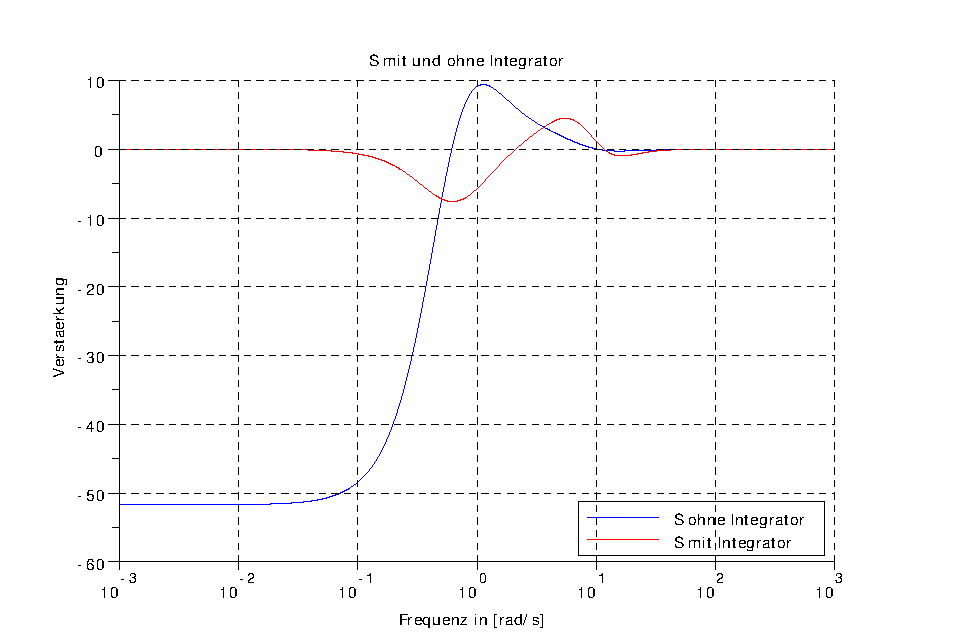
\includegraphics[scale=0.7, trim = 0cm 0cm 0cm 0cm, clip]{./Bilder/smitundohneIntegrator}
                \caption{S mit und ohne Integrator}
        \end{figure}
        
        Es lässt sich sehr schön erkennen, dass die Sensitivitätsfunktion des Regelkreises ohne Integrator eine Wert
        $\neq 0$ hat während die Sensitivitätsfunktion des Regelkreises mit Integrator den Wert $0$ annimmt.
    
        \begin{figure}[H]
        \centering
            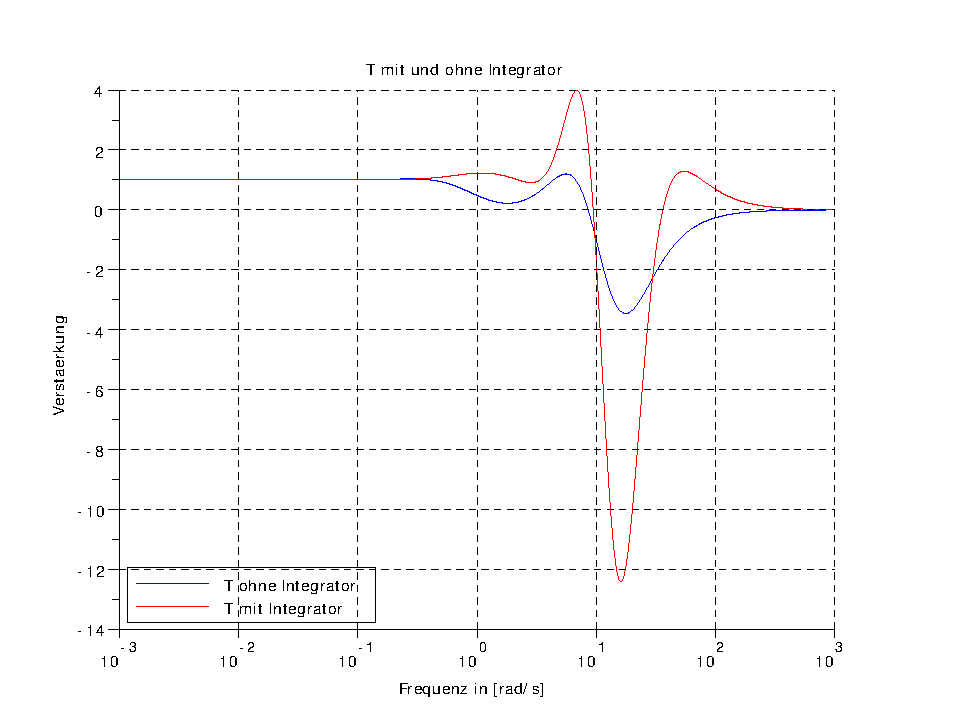
\includegraphics[scale=0.7, trim = 0cm 0cm 0cm 0cm, clip]{./Bilder/TmitundohneIntegrator}
                \caption{T mit und ohne Integrator}
        \end{figure}        
        
        Der Integrator hat zwar auch auf die komplimentäre Sensitivitätsfunktion einen Einfluss, jedoch bleibt der Wert
        für $s \rightarrow 0$ gleich. Das zeigt, dass der Integrator auch keinen negativen Einfluss auf die
        Führungssprungantwort hat.
        
         \end{quote}  % Ende Subsection Empfindlichkeitsfunktion
    
\end{quote} %Ende Section Vorbereitungsaufgaben 

%--------------------------------------------------------------------
%--------------------------------------------------------------------





\section{Auswertung}
\begin{quote}
    
    \subsection{Simulation}
    \begin{quote}
        Die Xcos Simulation zeigt, dass unserer Regler schon für einen Winkel von $2,18^{\circ}$ mit eiener
        Wagengeschwindigkeit von $3,7 \frac{m}{s}$ nahe an die erlaubten $4\frac{m}{s}$ herankommt. Für $2,19^{\circ}$
        überschreitet er diesen Wert bereits.\\
        Daher ist der Einzugsbereich unseres Reglers $\pm 2,18^{\circ}$. Das ist zugegebenermaßen nicht besonders viel
        und spricht für einen nicht optimal dimensionieren Regler.
    \end{quote}% Simulation


    \subsection{Versuchsstand}
    \begin{quote}
        
        Um das Verhalten unserer Regler zu untersuchen haben wir sie am Prüfstand aufgespielt.\\
        Um das Pendel in den Einzugsbereich unserer Regler zu bringen wurde ein Aufschwingregler zu Hilfe genommen, der
        nach dem aufschwingen an unsere Regler übergeben hat.
        
        \subsubsection{Winkelregler}
        \begin{quote}
            
            Als erstes haben wir nur den inneren Winkelregler untersucht. Hierbei gab es wie erwartet Schwierigkeiten,
            da die zurücklegbare Strecke des Wagens am Versuchstand relativ klein ist und der Regler keine Positionsregelung
            hat. Der Regler achtet somit nicht darauf, dass er auf der kleinen Strecke bleibt und der Wagen fährt, wie in
            Abb. \ref{Winkelregler_Position} zu sehen, einfach in eine Richtung davon, kommt schnell ans Ende
            des Versuchsstandes und löst somit den Notausschalter aus. Um zu verhindern, dass der Wagen sich zu weit von der
            Mitte der Strecke entfernt haben wir per potentiometer einen von null verschiedenen Sollwinkel vorgegeben sobald der Wagen
            zu sehr in eine Richtung fuhr.
            Dieses nachregeln, was der Positionsregler später übernimmt, erwies sich allerdings als sehr schwierig, da
            es sehr schnelle und genaue Reaktionen erfordert. Außerdem hat unser Regler die Kontrolle meistens sehr nahe am
            Rand des Versuchsstandes übergeben bekommen und hatte somit wenig Platz den Winkel auf null zu regeln.\\
            Von den vielen Versuchen die wir durchgeführt haben, waren die folgenden Messwerte am aussagekräftigsten.
            \\
            
            \begin{figure}[H]
            \centering
                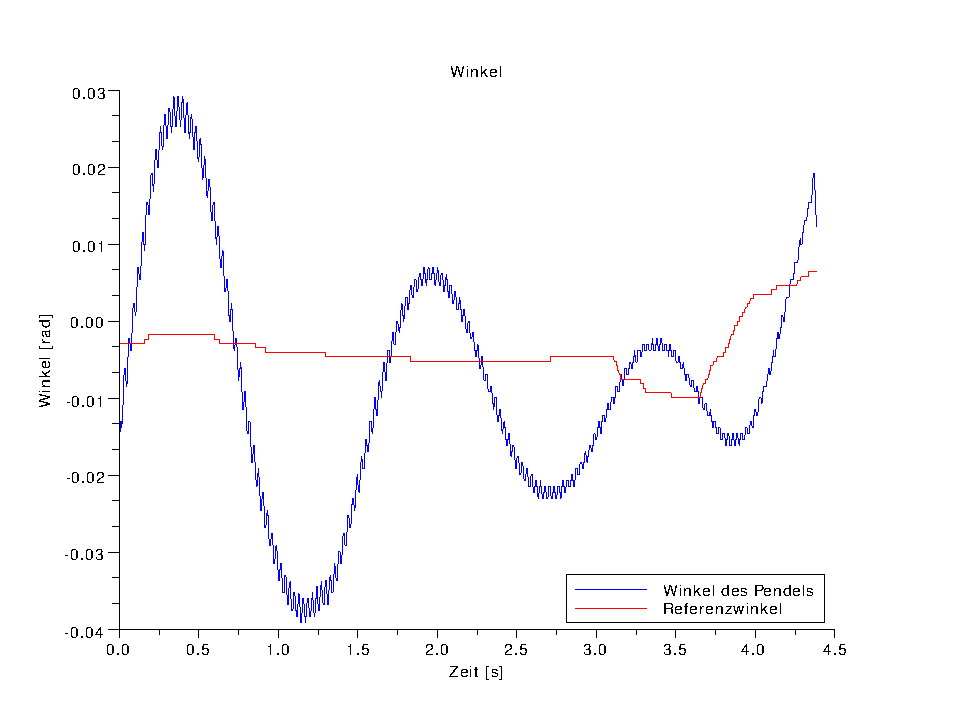
\includegraphics[scale=0.7, trim = 0cm 0cm 0cm 0cm, clip]{Bilder/win_win_ref}
                    \caption{ReferenzWinkel und Winkel des pendels}
                    \label{fig:win_win_ref}
            \end{figure}
            
            An der Grafik \ref{fig:win_win_ref} sieht man sehr schön, dass unser Regler das Pendel einfängt und
            stabilisiert. Bei ca. \SI{3,5}{\second} versuchen wir dann gegen zu reglen, weil der Wagen sich zu weit vom
            Mittelpunkt entfernt (siehe Abb. \ref{fig:win_pos}). Der Regler reagiert gut auf unsere Vorgabe, sie kam
            aber leider zu spät und der Wagen ist aus dem Messbereich herausgefahren.
            
            \begin{figure}[H]
            \centering
                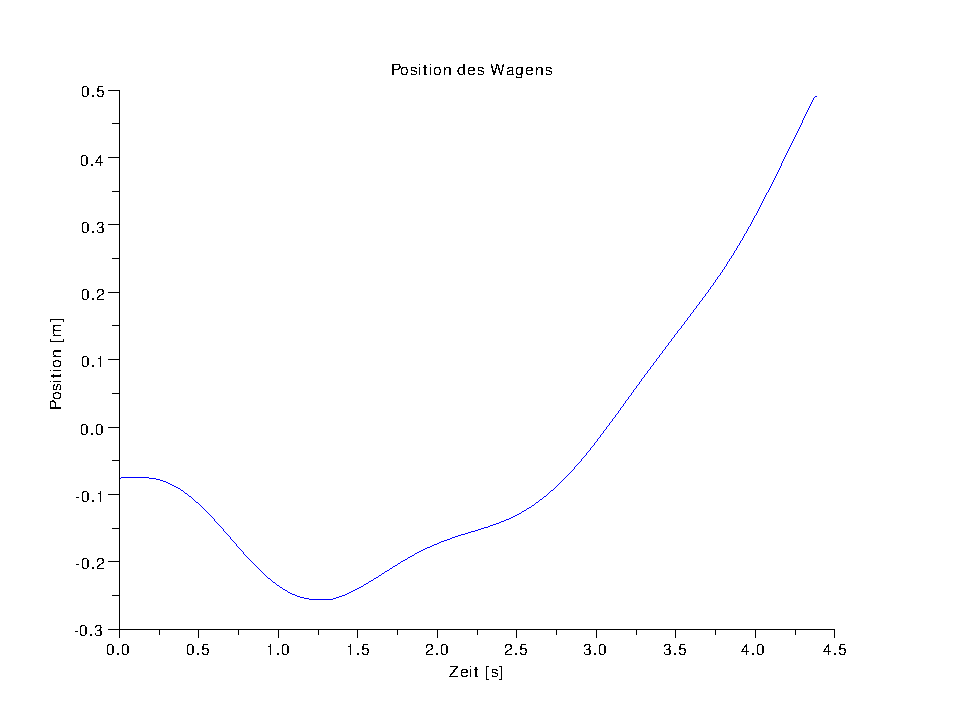
\includegraphics[scale=0.7, trim = 0cm 0cm 0cm 0cm, clip]{Bilder/win_pos}
                    \caption{Position des Wagens}
                    \label{fig:win_pos}
            \end{figure}
            
            \vspace{2em}
            
            Auch Geschwindigkeit des Wagens verhält sich wie erwartet:
            
            \begin{figure}[H]
            \centering
                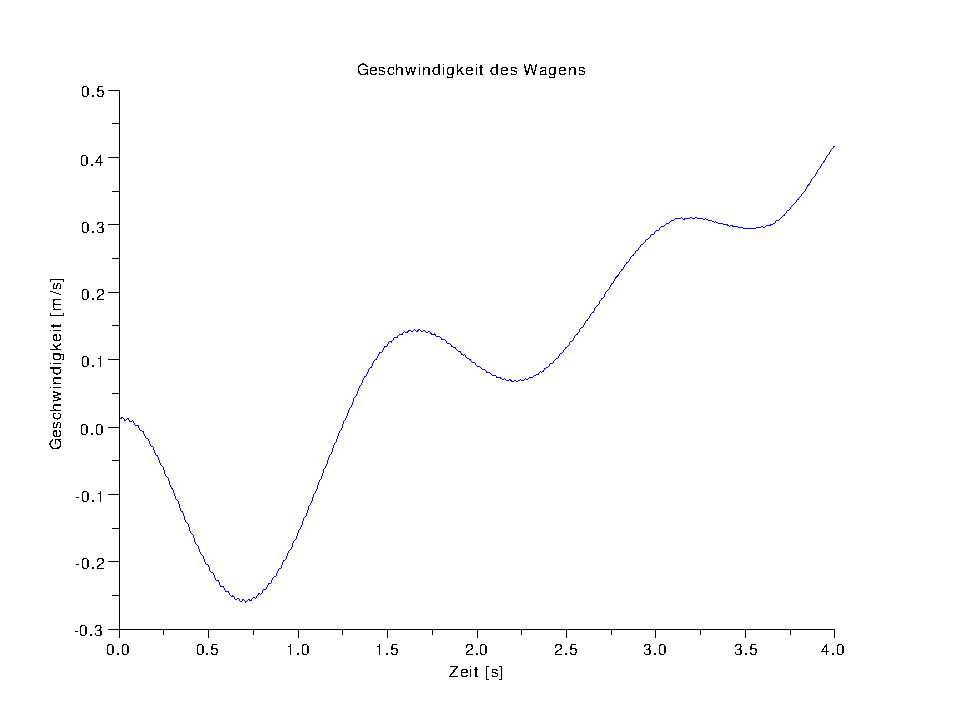
\includegraphics[scale=0.7, trim = 0cm 0cm 0cm 0cm, clip]{Bilder/win_gesch}
                    \caption{Geschwindigkeit des Wagens}
                    \label{fig:win_gesch}
            \end{figure}
            
            Wie schon in \ref{sec:Fuehrungsverhalten} Simuliert und erklärt nähert sich der Wagen einer konstanten
            Geschwindigkeit, da er davon aus geht keine beschränkung zu haben. 
            
            
            
        \end{quote}% Winkelregler
        
        \subsubsection{Positionsregler}
        \begin{quote}
            
            Als zweites haben wir noch den Positionsregler getestet. Wie in \ref{fig:pos_pos_ref} zu erkennen, hat es
            der Regler nach circa \SI{11}{\second} geschafft die Wagenposition aus zu regeln.\\
            Die Änderung der Position die wir nach \SI{15}{\second} durch das Potentiometer vorgegeben haben hat der
            Regler sehr gut umgesetzt.
            
            \begin{figure}[H]
                \centering
                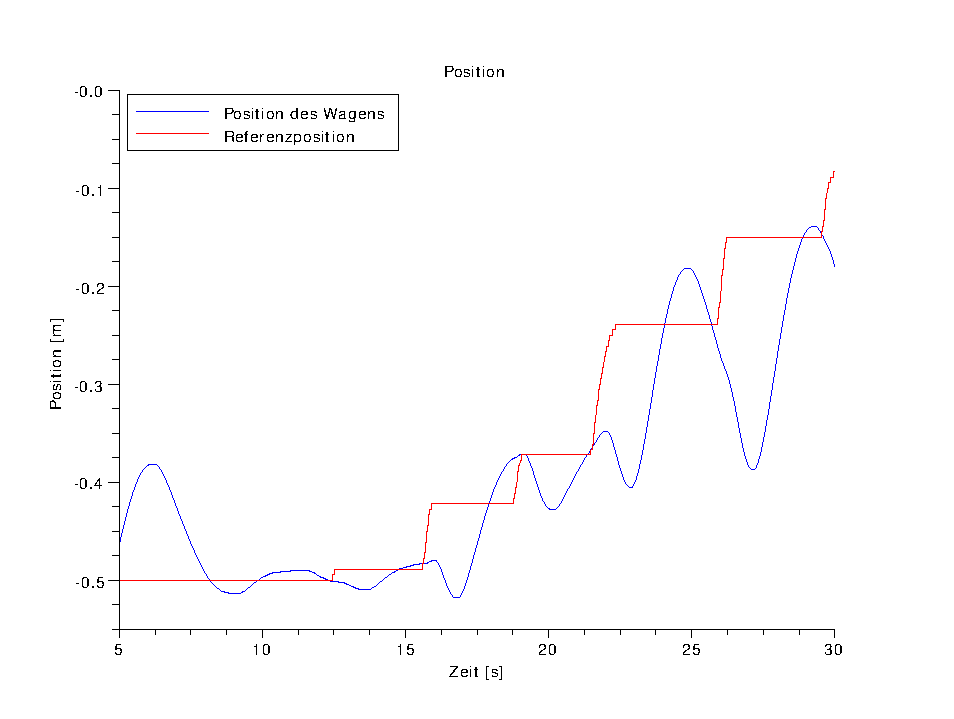
\includegraphics[scale=0.7, trim = 0cm 0cm 0cm 0cm, clip]{Bilder/pos_pos_ref}
                \caption{Position und Sollposition des Wagens}
                \label{fig:pos_pos_ref}
            \end{figure}
            
            Wie wir schon oben geschrieben haben waren unsere Regler offensichtlich nicht opimal dimensioniert, wesshalb
            das Pendel bei der Versuchsdurchführung nicht jedesmal gut ausgeregelt wurde. Das war auch der Grund
            wesshalb wir auch keine Störung auf das System aufnehmen und dementsprechend nicht disskutieren konnten.\\
            
            Opimierungspotential bestünde noch in der Geschwindigkeit beider Regler.\\
            Abgesehen davon haben beide Regler grundsätzlich funktioniert und Ergebnisse gelieftert, die unseren
            Erwartungen entspachen.
            
        \end{quote}% Positionsregler
        
    \end{quote}% Versuchsstand
    
    
\end{quote} %Ende Section Ergebnisse



%--------------------------------------------------------------------
%--------------------------------------------------------------------

\section{Scilabcode}
\begin{quote}
\begin{quote}
    \lstinputlisting[
        caption={Scilab-script},
        language=scilab,
        label=lst:scilab]
        {./Scilab/Pendel2a.sce}
        
    \lstinputlisting[
        caption={Polvorgabe-script},
        language=scilab,
        label=lst:scilab]
        {./Scilab/polvorgabe.sci}
    \lstinputlisting[
        caption={auswertung winkel},
        language=scilab,
        label=lst:scilab]
        {./Scilab/auswertung_winkel.sce}
    \lstinputlisting[
        caption={auswertung position},
        language=scilab,
        label=lst:scilab]
        {./Scilab/auswertung_position.sce}

\end{quote}

	
\end{quote} %Ende section

%--------------------------------------------------------------------
%--------------------------------------------------------------------    


%\begin{thebibliography}{999}
%\bibitem {Ueberschwingweite} Prof. Dr.-Ing. Raisch, Jörg; Dipl.-Ing. Hess, Anne-Katrin; Dipl.-Ing. Seel, Thomas:
%Grundlagen der Regelungstechnik - 4.Praktikum, S.5
%\bibitem {Ausregelzeit} Prof. Dr.-Ing. Raisch, Jörg; Dipl.-Ing. Hess, Anne-Katrin; Dipl.-Ing. Seel, Thomas:
%Grundlagen der Regelungstechnik - 4.Praktikum, S.5

%\usepackage{url}


%\bibitem{krachler}Christian Krachler:
%\href{http://www.krachler.com/fileadmin/user_upload/arbeiten/Reglersynthese_Christian_Krachler.pdf}{Reglersynthese nach
% dem Frequenzkennlinienverfahren}, S16, S22, 08.05.2012

%http://krachler.com/fileadmin/user\_upload/arbeiten/Reglersynthese\_Christian\_Krachler.pdf


%Name, Vorname.; evtl. Name2, Vorname2.: Titel des Dokumentes
%oder Buches, Zeitschrift/Verlag/URL (Auflage, Erscheinungsort, -jahr), ggf. Seitenzahlen
%\bibitem [Wiki10] {DigitaleMesskette2} \url{www.wikipedia.org}, Zugriff 22.03.2010
%\end{thebibliography}


\end{document}
